% Options for packages loaded elsewhere
\PassOptionsToPackage{unicode}{hyperref}
\PassOptionsToPackage{hyphens}{url}
%
\documentclass[
]{book}
\usepackage{amsmath,amssymb}
\usepackage{iftex}
\ifPDFTeX
  \usepackage[T1]{fontenc}
  \usepackage[utf8]{inputenc}
  \usepackage{textcomp} % provide euro and other symbols
\else % if luatex or xetex
  \usepackage{unicode-math} % this also loads fontspec
  \defaultfontfeatures{Scale=MatchLowercase}
  \defaultfontfeatures[\rmfamily]{Ligatures=TeX,Scale=1}
\fi
\usepackage{lmodern}
\ifPDFTeX\else
  % xetex/luatex font selection
\fi
% Use upquote if available, for straight quotes in verbatim environments
\IfFileExists{upquote.sty}{\usepackage{upquote}}{}
\IfFileExists{microtype.sty}{% use microtype if available
  \usepackage[]{microtype}
  \UseMicrotypeSet[protrusion]{basicmath} % disable protrusion for tt fonts
}{}
\makeatletter
\@ifundefined{KOMAClassName}{% if non-KOMA class
  \IfFileExists{parskip.sty}{%
    \usepackage{parskip}
  }{% else
    \setlength{\parindent}{0pt}
    \setlength{\parskip}{6pt plus 2pt minus 1pt}}
}{% if KOMA class
  \KOMAoptions{parskip=half}}
\makeatother
\usepackage{xcolor}
\usepackage{color}
\usepackage{fancyvrb}
\newcommand{\VerbBar}{|}
\newcommand{\VERB}{\Verb[commandchars=\\\{\}]}
\DefineVerbatimEnvironment{Highlighting}{Verbatim}{commandchars=\\\{\}}
% Add ',fontsize=\small' for more characters per line
\usepackage{framed}
\definecolor{shadecolor}{RGB}{248,248,248}
\newenvironment{Shaded}{\begin{snugshade}}{\end{snugshade}}
\newcommand{\AlertTok}[1]{\textcolor[rgb]{0.94,0.16,0.16}{#1}}
\newcommand{\AnnotationTok}[1]{\textcolor[rgb]{0.56,0.35,0.01}{\textbf{\textit{#1}}}}
\newcommand{\AttributeTok}[1]{\textcolor[rgb]{0.13,0.29,0.53}{#1}}
\newcommand{\BaseNTok}[1]{\textcolor[rgb]{0.00,0.00,0.81}{#1}}
\newcommand{\BuiltInTok}[1]{#1}
\newcommand{\CharTok}[1]{\textcolor[rgb]{0.31,0.60,0.02}{#1}}
\newcommand{\CommentTok}[1]{\textcolor[rgb]{0.56,0.35,0.01}{\textit{#1}}}
\newcommand{\CommentVarTok}[1]{\textcolor[rgb]{0.56,0.35,0.01}{\textbf{\textit{#1}}}}
\newcommand{\ConstantTok}[1]{\textcolor[rgb]{0.56,0.35,0.01}{#1}}
\newcommand{\ControlFlowTok}[1]{\textcolor[rgb]{0.13,0.29,0.53}{\textbf{#1}}}
\newcommand{\DataTypeTok}[1]{\textcolor[rgb]{0.13,0.29,0.53}{#1}}
\newcommand{\DecValTok}[1]{\textcolor[rgb]{0.00,0.00,0.81}{#1}}
\newcommand{\DocumentationTok}[1]{\textcolor[rgb]{0.56,0.35,0.01}{\textbf{\textit{#1}}}}
\newcommand{\ErrorTok}[1]{\textcolor[rgb]{0.64,0.00,0.00}{\textbf{#1}}}
\newcommand{\ExtensionTok}[1]{#1}
\newcommand{\FloatTok}[1]{\textcolor[rgb]{0.00,0.00,0.81}{#1}}
\newcommand{\FunctionTok}[1]{\textcolor[rgb]{0.13,0.29,0.53}{\textbf{#1}}}
\newcommand{\ImportTok}[1]{#1}
\newcommand{\InformationTok}[1]{\textcolor[rgb]{0.56,0.35,0.01}{\textbf{\textit{#1}}}}
\newcommand{\KeywordTok}[1]{\textcolor[rgb]{0.13,0.29,0.53}{\textbf{#1}}}
\newcommand{\NormalTok}[1]{#1}
\newcommand{\OperatorTok}[1]{\textcolor[rgb]{0.81,0.36,0.00}{\textbf{#1}}}
\newcommand{\OtherTok}[1]{\textcolor[rgb]{0.56,0.35,0.01}{#1}}
\newcommand{\PreprocessorTok}[1]{\textcolor[rgb]{0.56,0.35,0.01}{\textit{#1}}}
\newcommand{\RegionMarkerTok}[1]{#1}
\newcommand{\SpecialCharTok}[1]{\textcolor[rgb]{0.81,0.36,0.00}{\textbf{#1}}}
\newcommand{\SpecialStringTok}[1]{\textcolor[rgb]{0.31,0.60,0.02}{#1}}
\newcommand{\StringTok}[1]{\textcolor[rgb]{0.31,0.60,0.02}{#1}}
\newcommand{\VariableTok}[1]{\textcolor[rgb]{0.00,0.00,0.00}{#1}}
\newcommand{\VerbatimStringTok}[1]{\textcolor[rgb]{0.31,0.60,0.02}{#1}}
\newcommand{\WarningTok}[1]{\textcolor[rgb]{0.56,0.35,0.01}{\textbf{\textit{#1}}}}
\usepackage{longtable,booktabs,array}
\usepackage{calc} % for calculating minipage widths
% Correct order of tables after \paragraph or \subparagraph
\usepackage{etoolbox}
\makeatletter
\patchcmd\longtable{\par}{\if@noskipsec\mbox{}\fi\par}{}{}
\makeatother
% Allow footnotes in longtable head/foot
\IfFileExists{footnotehyper.sty}{\usepackage{footnotehyper}}{\usepackage{footnote}}
\makesavenoteenv{longtable}
\usepackage{graphicx}
\makeatletter
\def\maxwidth{\ifdim\Gin@nat@width>\linewidth\linewidth\else\Gin@nat@width\fi}
\def\maxheight{\ifdim\Gin@nat@height>\textheight\textheight\else\Gin@nat@height\fi}
\makeatother
% Scale images if necessary, so that they will not overflow the page
% margins by default, and it is still possible to overwrite the defaults
% using explicit options in \includegraphics[width, height, ...]{}
\setkeys{Gin}{width=\maxwidth,height=\maxheight,keepaspectratio}
% Set default figure placement to htbp
\makeatletter
\def\fps@figure{htbp}
\makeatother
\setlength{\emergencystretch}{3em} % prevent overfull lines
\providecommand{\tightlist}{%
  \setlength{\itemsep}{0pt}\setlength{\parskip}{0pt}}
\setcounter{secnumdepth}{5}
\ifLuaTeX
  \usepackage{selnolig}  % disable illegal ligatures
\fi
\IfFileExists{bookmark.sty}{\usepackage{bookmark}}{\usepackage{hyperref}}
\IfFileExists{xurl.sty}{\usepackage{xurl}}{} % add URL line breaks if available
\urlstyle{same}
\hypersetup{
  pdftitle={Applied Statistics in Environment and Ecology},
  pdfauthor={Dr.~Brad Fedy},
  hidelinks,
  pdfcreator={LaTeX via pandoc}}

\title{Applied Statistics in Environment and Ecology}
\author{Dr.~Brad Fedy}
\date{2024-01-06}

\begin{document}
\maketitle

{
\setcounter{tocdepth}{1}
\tableofcontents
}
\hypertarget{welcome}{%
\chapter{Welcome}\label{welcome}}

This book is being written to support student progress and learning in ERS 669 Applied Statistics in Environment and Ecology. Notice the present tense in the previous sentence. This book is a work in progress. The book is written using \href{https://bookdown.org/}{Bookdown} which is a package in R that facilitates writing books with R Markdown. The book is provided as .HTML files on LEARN. This allows for a dynamic document allowing you to easily navigate through book sections and copy code. The book files will be updated on LEARN each week in preparation for our in-class programming sessions.

\hypertarget{introduction-to-r}{%
\chapter{Introduction to R}\label{introduction-to-r}}

\hypertarget{what-is-r}{%
\section{What is R?}\label{what-is-r}}

R is a programming language and software environment for statistical computing and graphics created by Ross Ihaka and Robert GentlemanIhaka R. \& Gentleman R. 1996. R: a language for data analysis and graphics. Journal of Computational and Graphical Statistics 5: 299-314. The development and distribution of R is carried out by a group of statisticians known as the R Development Core Team and is distributed under the terms of the GNU Public License. Thus, R can be freely downloaded from the Comprehensive R Archive Network (CRAN) \href{http://www.r-project.org}{website}. The fact that R is free and available across operating systems is one of the main benefits of learning and using R for statistical analysis. There are multiple other freely available programming languages and software what can be used for statistics and data science (e.g., \href{https://www.python.org/}{Python}), but R is one of the most common for applications in academia and in ecology and environmental studies, specifically. Additionally, there are many commercial statistical packages that are comparable and can be used to similar ends; but, at a cost \textgreater{} \$1,000 per license.

Installation of R software is straight forward for all major platforms and instructions are provided on the website. Most of the analyses and tasks that are conducted in R are done through the command-line interface and thus, for the non-programmer the learning curve for this software may be steeper than for most point and click statistical programs. There are, however, several advantages of using R and the command-line setup that make putting the effort into learning this program well worth your time:

\begin{itemize}
\item
  \textbf{Cost:} It's free! No matter what lab, agency, or company you work with, R can go with you.
\item
  \textbf{Simplicity:} R is a relatively simple programming language, allowing you to accomplish a lot with minimal lines of code.
\item
  \textbf{Diverse and continued package development:} In the past, researchers have needed to learn multiple software packages to conduct their analyses and display their results. Because R is open source and relies on user contributed \texttt{packages}, a wide variety of general and specialized analyses and plotting functions can be conducted in R. New \texttt{packages} are developed and existing ones are updated each day. This reduces this need to learn multiple software packages.
\item
  \textbf{Integration:} R works nicely with other scripting languages and open source software used for a variety of tasks, including Geographic Information Systems (e.g., \href{http://grass.osgeo.org}{GRASS}, \href{http://www.qgis.org}{QGIS}) and document production (e.g., \href{https://www.markdownguide.org/}{Markdown} - more on this later).
\item
  \textbf{Reproducibility:} If used properly, command-line scripting keeps detailed records of your analyses. This makes is easy to share, repeat, and modify your work. \emph{This is an important point}. One of the most important components of good science is replicability. Most research requires many steps from organizing and checking the data to conducting the analysis. Using statistical software that allows you to point and click through your analysis does not usually leave any record of what has been done. Thus, it can be difficult to remember and precisely replicate the data manipulation and analyses. Using command-line scripting requires the analyst to type out a line of code for every action they want to perform. Use of a code hosting platform such as \href{https://github.com/}{GitHub} can further facilitate transparency, reproducibility, version control, and collaboration. We will not cover the use of \href{https://github.com/}{GitHub} explicitly in this course, but it is a potentially useful tool you may encounter as you progress through your research.
\item
  \textbf{Self-education:} There is a large, active, and (mostly) helpful community of people dedicated to education and training in R programming languages. With enough effort you can find online tutorials or examples for any statistical analysis in R, along with example code. This community is one that you will rely on throughout your R programming and statistical education.
\end{itemize}

This manual will serve multiple purposes. It will be used to provide examples during lectures and code that you will be required to work through on you own. The introduction to R will be brief so that we can get into working with data as quickly as possible. However, there are many excellent resources to facilitate your R-based education. \emph{Do not fall behind in your understanding of R}. Ask frequent questions of Dr.~Fedy and your colleagues. Be sure you understand each line of code. We will use R for all course topics. It is essential that you understand the code in order to understand the data management and statistics that are the focus of the course.

This manual is not intended to turn you all into R programming ninjas and statisticians. The intention is to provide you with the tools required for self-education. R is a potentially relevant tool for anyone who uses numbers to understand the world - regardless of your area of interest. When programming in R, there are often multiple ways to solve the same problem. That is part of the fun and challenge of programming. Of course, the different options to completing an analysis increase with increasing complexity of the problem; for simple problems there are usually only a few ways to solve it, for complex problems there are often many ways to solve it. Throughout the course I will demonstrate the code and approaches that have worked for me, my students, and collaborators. However, I intentionally do not provide all the answers and you will need to problem-solve and self-educate in order to successfully complete all the assignments.

You will need to install two pieces of software on your computer: \href{https://www.r-project.org/}{R} and \href{https://www.r-project.org/}{RStudio}. Both of these are free to download. When you open R, you will see the basic command-line console version of R. RStudio is an Integrated Development Environment (IDE) for R, that provides a few more bells and whistles and tends to ease the introduction to R. You do not \emph{have to} use RStudio, but it is highly recommended.

\hypertarget{rstudio}{%
\section{RStudio}\label{rstudio}}

One of the most significant advantages of using the command-line structure in R is that, if done properly, you have detailed documentation for everything that you do. This allows you to easily change, manipulate, and share your code with others. This process is facilitated by writing any code you use into a script file, instead of entering it directly into R. \href{http://www.rstudio.com/ide/}{Rstudio} can be customized in many ways, but is typically divided into four windows and that provide simultaneous views of important information. The most frequently used windows and tabs are:

\textbf{scripts:} Write your code here for a permanent record.

\textbf{console:} Essentially R running within RStudio. Displays output and any errors.

\textbf{Environment/Plots:} Environment shows you the objects that are currently saved in your workspace and Plots displays any plots that you create.

\textbf{History/Files/Packages:} These tabs are less commonly referenced and are fairly self-explanatory.

\hypertarget{before-you-begin}{%
\section{Before you begin}\label{before-you-begin}}

There are four important things that you should note about R and this manual that will help you as you work through the instructions and exercises:

\begin{itemize}
\item
  Throughout this book R code is in the grey boxes, with results that you should see in R following this text prefaced by \texttt{\#\#}. Text following a \texttt{\#} are not read by R and are used to comment the code. I use \texttt{\#} marks to provide information about a particular command or function.
\item
  When working in the R console, the up and down arrows can be used to retrieve past commands, saving you from re-typing it.
\item
  If you see a \texttt{+} prompt, it means R is waiting for more input. Often this means that you have forgotten a closing parenthesis or made some other syntax error. If you cannot figure out its meaning, hit the escape key and start the command fresh.
\item
  In R, tasks such as calculating means, conducting statistical analysis or generating plots are completed through the use of functions. A function in mathematics is something that relates an input to an output. It has three basic components an input, a relationship, an output. The function defines the relationship. The arguments are the variables or inputs required for the function to produce the desired output. For example, a function to calculate the mean height of everyone in the class would require 1 argument: the height of each person. The function calculates the number of people (n) based on the number of observations and outputs the mean by summing all individual heights and dividing by n.~We will go through many examples of functions throughout the course. Functions in R accept arguments, which are used to complete the task (produce output) and use the following syntax: \texttt{\textgreater{}\ functionname(argument\ 1,\ argument\ 2,\ ...)}
\item
  The arguments are always surrounded by (round) parentheses and separated by commas. Some functions (e.g., \texttt{data()}) have no required arguments, but you still need the parentheses.
\item
  If you type a function name without the parentheses, you will see the code that is the basis for that function including the required arguments.
\item
  Before you begin any analysis it is important that you tell R the home directory that you will be working in by using the command \texttt{setwd(“path\ to\ folder”)}. It is important that you include the quotation marks (``\,'') around the pathname. It is also important that you have write access to the drive that you are using for your working directory. Please keep this in mind if you are using multiple computers. You can set your working directory using the drop down menus in RStudio, by typing out the path manually, or by using the command \texttt{file.choose()}.
\end{itemize}

\hypertarget{setting-a-working-directory}{%
\section{Setting a working directory}\label{setting-a-working-directory}}

The first steps for setting a working director typically happen outside of R or RStudio. The first step is to create a new folder on your computer where you want to store all of the work associated with this class or with a particular assignment. Once the folder is created, the second step is to put a file into the folder you created. It does not matter what type of file you put in this folder. Typically, I use a simple blank .txt or the data file (typically .csv) file for examples in class. Once this is complete navigate back to R and type in the following command at the prompt:

\begin{Shaded}
\begin{Highlighting}[]
\FunctionTok{file.choose}\NormalTok{()}
\end{Highlighting}
\end{Shaded}

R will then open your computers file management and navigation system. For Mac OS this is Finder, in Windows machines, the Explorer window will open. Within that window, navigate to the working folder you just created and the file you put in it. Then select (``choose'') that file. R will respond by putting the entire path name into your R console window.

\begin{verbatim}
[1] "/Users/bfedy/Documents/PROJECTS/Rwork/Anything filename.txt"
\end{verbatim}

Select everything in the path except for the file name (e.g., the .txt file) and copy and paste it into your setwd command.

\begin{Shaded}
\begin{Highlighting}[]
\FunctionTok{setwd}\NormalTok{(}\StringTok{"/Users/bfedy/Documents/PROJECTS/Rwork/"}\NormalTok{)}
\end{Highlighting}
\end{Shaded}

Once this is completed R will put everything it generates and look for any files you pass to it in the ``Rwork'' file that I created above. Please note: the path names will be different on every computer that you use, so you will need to reset the working director every time you change computers.

\hypertarget{getting-help-in-r}{%
\section{Getting help in R}\label{getting-help-in-r}}

The list of functions available within R is much too great to provide even an adequate summary. There are, however, a wide variety of online resources available that we expect you to draw on throughout this course. Searching ``R'' and ``Type of analysis'' in a search engine will often produce code and sometimes tutorials for the analyses you are looking to undertake. To be more specific, you can also include ``cran'' as a keyword. As you work through this manual and your assignments I encourage you to start a document where you note commands that you find useful with a brief description. This will help save you from learning the same command multiple times. You are learning a new language, please take notes and do not expect yourself to remember everything. You might want to check out some \href{http://r-dir.com/reference/crib-sheets.html\%7C\%7Chttp://r-dir.com/reference/crib-sheets.html}{cheat sheets} compiled by R as examples. There are also a variety of ways to get help within the R software. If you type a \texttt{?} followed by the command or \texttt{help(commandname)} will pull up a help file document with the follow structure:

\textbf{Description:} Brief description.

\textbf{Usage:} For a function, gives the name with all its arguments and the possible options (with the corresponding default values); for an operator gives the typical use.

\textbf{Arguments:} For a function, details each of its arguments.

\textbf{Details:} Detailed description.

\textbf{Value:} If applicable, the type of object returned by the function or the operator.

\textbf{See Also:} Other help pages close or similar to the present one.

\textbf{Examples:} Some working examples of the function or operator.

Other methods for obtaining help when you do not know the exact name of the command you are looking for is to use \texttt{??} or \texttt{help.search} with a key word. This will give a list of commands with topics that match your key word.

Expect to spend a good amount of time searching for help on the internet while you are programming - particularly at the beginning. It is common to spend as much time (or more) searching the internet as you spend writing code when first starting out. There are many excellent websites and free resources for help and guidance through your R and statistical journey. I cannot list them all here; however, two books that I go back to regularly for R programming help are:

\href{https://r4ds.hadley.nz/}{R for Data Science}\li

\href{https://r-graphics.org/}{R Graphics Cookbook}\li

\hypertarget{defining-r-objects}{%
\section{Defining R objects}\label{defining-r-objects}}

A fundamental concept of R is that when R is running, data and results are stored in the active memory in the form of objects, which are all assigned a name by the user. The user can then manipulate these objects through the use of \emph{operators} or \emph{functions}. \emph{Operators} perform tasks including arimetic, logical, and conditional actions. \emph{Functions} are the work horses of R and are self-contained modules of code that accomplish a specific task. Functions are typically provided data (i.e., values, vectors, dataframes), process that data according to the rules defined in the function, and return a result. Functions can be user-generated, but the majority of functions that you use will be contained within R \texttt{packages}. Much more information will be presented on both these topics throughout the book. Objects can be stored in a variety of ways and it is critical to understand how objects are created, their formats, and what they mean as a first step in learning R. The most basic form of an object is a scalar (i.e., single value), which can be creating using the ``assign'' \texttt{\textless{}-} operator. The assign operator is simply a less than sign followed by a minus sign. The following examples demonstrate the basics.

\begin{Shaded}
\begin{Highlighting}[]
\NormalTok{n }\OtherTok{\textless{}{-}} \DecValTok{15}
\NormalTok{n}
\end{Highlighting}
\end{Shaded}

\begin{verbatim}
## [1] 15
\end{verbatim}

\begin{Shaded}
\begin{Highlighting}[]
\NormalTok{n }\OtherTok{\textless{}{-}} \StringTok{"Applied Statistics"}
\NormalTok{n}
\end{Highlighting}
\end{Shaded}

\begin{verbatim}
## [1] "Applied Statistics"
\end{verbatim}

\begin{Shaded}
\begin{Highlighting}[]
\NormalTok{N }\OtherTok{\textless{}{-}} \DecValTok{18}
\end{Highlighting}
\end{Shaded}

Two things of particular note in the example above, 1) R is case sensitive with \texttt{n} being different than \texttt{N}, and 2) if an object exists and is assigned a new name, the previous value is erased without any warning. Thus, it is important to pay attention to the variables you create and those which are already stored in your active memory. You can get a list of the names of variables in memory with the \texttt{ls()} command or for the variables with some details on the objects use \texttt{ls.str()}. In RStudio, you can also see all the objects you have created in the `Environment' tab. To remove objects from the active memory you can use the \texttt{rm(\textquotesingle{}object\textquotesingle{})} command. Look at the example below and note that we use \texttt{rm(list=ls())} to list and remove all objects in the active memory. It is good practice to start all of your new scripts with the \texttt{rm(list=ls()} command. That way you know the script is not dependent on any objects previously stored in your Environment (i.e., working memory). When you run the code below, you will see the corresponding values show up in R console. If you want to save those values for later use, you will need to assign them an object name.

\begin{Shaded}
\begin{Highlighting}[]
\NormalTok{Y }\OtherTok{\textless{}{-}} \FunctionTok{c}\NormalTok{(}\DecValTok{2}\NormalTok{,}\DecValTok{2}\NormalTok{,}\DecValTok{3}\NormalTok{,}\DecValTok{5}\NormalTok{,}\DecValTok{6}\NormalTok{,}\DecValTok{7}\NormalTok{,}\DecValTok{10}\NormalTok{,}\DecValTok{11}\NormalTok{,}\DecValTok{11}\NormalTok{,}\DecValTok{12}\NormalTok{)  }\CommentTok{\# create a vector of these numbers}
\NormalTok{Y[}\DecValTok{4}\NormalTok{]  }\CommentTok{\# select the fourth value}
\end{Highlighting}
\end{Shaded}

\begin{verbatim}
## [1] 5
\end{verbatim}

\begin{Shaded}
\begin{Highlighting}[]
\NormalTok{Y[}\DecValTok{1}\SpecialCharTok{:}\DecValTok{5}\NormalTok{]  }\CommentTok{\# select the first five values}
\end{Highlighting}
\end{Shaded}

\begin{verbatim}
## [1] 2 2 3 5 6
\end{verbatim}

\begin{Shaded}
\begin{Highlighting}[]
\NormalTok{Y[}\DecValTok{5}\SpecialCharTok{:}\DecValTok{10}\NormalTok{]  }\CommentTok{\# select the last five values}
\end{Highlighting}
\end{Shaded}

\begin{verbatim}
## [1]  6  7 10 11 11 12
\end{verbatim}

To select or identify values within two dimensional data such as matrices and data frames you will need two numbers (separated by a comma) in the square brackets. The first number specifies the row or range of rows, and the second number specifies the column or range of columns (Dr.~Fedy finds it helpful to think of RC Cola to remember the order: rows, then columns. You may not have heard of RC Cola, but you get the point, think of something meaningful to you). For data frames you may also want to extract the column headers of names of columns, which you can replace if you wish to change the name of one or more columns. Below are some examples executed using base R. There are multiple packages that make the selection of data and values more intuitive (much more on those later).

\begin{Shaded}
\begin{Highlighting}[]
\CommentTok{\# Set up a 2 dimensional data frame}
\FunctionTok{options}\NormalTok{(}\AttributeTok{digits =} \DecValTok{3}\NormalTok{)  }\CommentTok{\# set significant digits in R}
\NormalTok{snake.df }\OtherTok{\textless{}{-}} \FunctionTok{data.frame}\NormalTok{(}\AttributeTok{species =} \FunctionTok{rep}\NormalTok{(}\StringTok{"P.gloydi"}\NormalTok{, }\DecValTok{20}\NormalTok{), }
                       \AttributeTok{sex =} \FunctionTok{factor}\NormalTok{(}\FunctionTok{rep}\NormalTok{(}\FunctionTok{c}\NormalTok{(}\StringTok{"male"}\NormalTok{, }\StringTok{"female"}\NormalTok{),}\DecValTok{10}\NormalTok{)),}
                       \AttributeTok{mass =} \FunctionTok{runif}\NormalTok{(}\AttributeTok{n=}\DecValTok{20}\NormalTok{, }\AttributeTok{min=}\FloatTok{0.5}\NormalTok{, }\AttributeTok{max=}\FloatTok{1.5}\NormalTok{),}
                       \AttributeTok{length =} \FunctionTok{runif}\NormalTok{(}\AttributeTok{n=}\DecValTok{20}\NormalTok{, }\AttributeTok{min=}\DecValTok{50}\NormalTok{, }\AttributeTok{max=}\DecValTok{100}\NormalTok{))}
\NormalTok{snake.df}
\end{Highlighting}
\end{Shaded}

\begin{verbatim}
##     species    sex  mass length
## 1  P.gloydi   male 1.160   71.3
## 2  P.gloydi female 0.693   75.6
## 3  P.gloydi   male 0.930   57.0
## 4  P.gloydi female 0.710   59.8
## 5  P.gloydi   male 0.618   58.0
## 6  P.gloydi female 0.994   89.8
## 7  P.gloydi   male 1.053   94.0
## 8  P.gloydi female 0.809   53.2
## 9  P.gloydi   male 0.970   75.4
## 10 P.gloydi female 1.400   79.5
## 11 P.gloydi   male 1.053   55.6
## 12 P.gloydi female 1.409   80.7
## 13 P.gloydi   male 0.888   64.2
## 14 P.gloydi female 1.145   82.4
## 15 P.gloydi   male 1.181   68.7
## 16 P.gloydi female 0.606   94.4
## 17 P.gloydi   male 0.708   68.8
## 18 P.gloydi female 0.989   66.6
## 19 P.gloydi   male 0.853   78.5
## 20 P.gloydi female 1.345   63.7
\end{verbatim}

Be sure that you understand what is happening in each of the lines of code above. This would be a good time to use the help functions in R to help you understand.

\begin{Shaded}
\begin{Highlighting}[]
\CommentTok{\# The output from the following code will show up in your R console}
\FunctionTok{names}\NormalTok{(snake.df)  }\CommentTok{\# extract names of columns}
\end{Highlighting}
\end{Shaded}

\begin{verbatim}
## [1] "species" "sex"     "mass"    "length"
\end{verbatim}

\begin{Shaded}
\begin{Highlighting}[]
\NormalTok{snake.df[ , }\DecValTok{1}\NormalTok{]  }\CommentTok{\# extract the first column (note: the space are not necessary)}
\end{Highlighting}
\end{Shaded}

\begin{verbatim}
##  [1] "P.gloydi" "P.gloydi" "P.gloydi" "P.gloydi" "P.gloydi" "P.gloydi"
##  [7] "P.gloydi" "P.gloydi" "P.gloydi" "P.gloydi" "P.gloydi" "P.gloydi"
## [13] "P.gloydi" "P.gloydi" "P.gloydi" "P.gloydi" "P.gloydi" "P.gloydi"
## [19] "P.gloydi" "P.gloydi"
\end{verbatim}

\begin{Shaded}
\begin{Highlighting}[]
\NormalTok{snake.df[}\DecValTok{1}\NormalTok{, ]  }\CommentTok{\# extract the first row}
\end{Highlighting}
\end{Shaded}

\begin{verbatim}
##    species  sex mass length
## 1 P.gloydi male 1.16   71.3
\end{verbatim}

\begin{Shaded}
\begin{Highlighting}[]
\NormalTok{snake.df[ , }\DecValTok{1}\SpecialCharTok{:}\DecValTok{3}\NormalTok{]  }\CommentTok{\# extract the first 3 columns}
\end{Highlighting}
\end{Shaded}

\begin{verbatim}
##     species    sex  mass
## 1  P.gloydi   male 1.160
## 2  P.gloydi female 0.693
## 3  P.gloydi   male 0.930
## 4  P.gloydi female 0.710
## 5  P.gloydi   male 0.618
## 6  P.gloydi female 0.994
## 7  P.gloydi   male 1.053
## 8  P.gloydi female 0.809
## 9  P.gloydi   male 0.970
## 10 P.gloydi female 1.400
## 11 P.gloydi   male 1.053
## 12 P.gloydi female 1.409
## 13 P.gloydi   male 0.888
## 14 P.gloydi female 1.145
## 15 P.gloydi   male 1.181
## 16 P.gloydi female 0.606
## 17 P.gloydi   male 0.708
## 18 P.gloydi female 0.989
## 19 P.gloydi   male 0.853
## 20 P.gloydi female 1.345
\end{verbatim}

\begin{Shaded}
\begin{Highlighting}[]
\NormalTok{snake.df[}\DecValTok{1}\SpecialCharTok{:}\DecValTok{4}\NormalTok{,}\DecValTok{1}\SpecialCharTok{:}\DecValTok{3}\NormalTok{]  }\CommentTok{\# extract the first 3 columns and 4 rows}
\end{Highlighting}
\end{Shaded}

\begin{verbatim}
##    species    sex  mass
## 1 P.gloydi   male 1.160
## 2 P.gloydi female 0.693
## 3 P.gloydi   male 0.930
## 4 P.gloydi female 0.710
\end{verbatim}

It is also possible using base R to call individual columns of a data frame using the names of the data frame and the column separated by a \texttt{\$}.

\begin{Shaded}
\begin{Highlighting}[]
\NormalTok{snake.df}\SpecialCharTok{$}\NormalTok{sex}
\end{Highlighting}
\end{Shaded}

\begin{verbatim}
##  [1] male   female male   female male   female male   female male   female
## [11] male   female male   female male   female male   female male   female
## Levels: female male
\end{verbatim}

\begin{Shaded}
\begin{Highlighting}[]
\NormalTok{snake.df}\SpecialCharTok{$}\NormalTok{length}
\end{Highlighting}
\end{Shaded}

\begin{verbatim}
##  [1] 71.3 75.6 57.0 59.8 58.0 89.8 94.0 53.2 75.4 79.5 55.6 80.7 64.2 82.4 68.7
## [16] 94.4 68.8 66.6 78.5 63.7
\end{verbatim}

\hypertarget{exporting-data-frames}{%
\section{Exporting data frames}\label{exporting-data-frames}}

As we alluded to earlier, in reality R's main function is for analyzing and graphing data, and different programs such as excel or other database programs will be used when collecting and entering data. Thus, being able to import and export data from R is essential. Here, we will first introduce you to the \texttt{write.table()} function, which is the primary function used to export a data fame. The main parameters that you need to be aware of are listed below, but you can use R help \texttt{?write.table} to get a list of all options and more information. One of the most important arguments in this function is the \texttt{sep} argument, which specifies how each column in the data frame will be separated. As a default, I tend to prefer the \texttt{sep=","} option which allows you to open your data a comma separated file (.csv) which is possible in most editors that you will want to use. If you do not provide a file name (as we do below) for the argument \texttt{file} then the output is printed to the screen. After you create the table below try opening it in a text editor or Excel (or some other spreadsheet software). Be sure you have set your working director \texttt{setwd("filename")} so you know where the output will be stored on your machine.

\begin{Shaded}
\begin{Highlighting}[]
\FunctionTok{write.table}\NormalTok{(snake.df, }\AttributeTok{sep=}\StringTok{","}\NormalTok{, }\AttributeTok{row.names=}\ConstantTok{FALSE}\NormalTok{, }\AttributeTok{col.names=}\ConstantTok{TRUE}\NormalTok{)}
\end{Highlighting}
\end{Shaded}

\hypertarget{installing-and-loading-packages}{%
\subsection{Installing and loading packages}\label{installing-and-loading-packages}}

An important component and one of the main advantages of R is that users can write and provide packages. These packages are essentially a series of functions that have been compiled together and can be loaded into R to make these functions available. Without installing and loading these packages these functions are not available. Loading packages in R can be done in R from the command-line if you know the package that you wish to install. Two packages that we will need in later models are the lattice and grid packages. These can be installed using the input below, with \texttt{dependencies=TRUE} specifying that you wish all packages that are needed to be installed at the same time. You may get a pop up window asking if you want to install these in a local directory. If so you should answer yes. You will likely also be asked to specify a CRAN mirror (i.e., download location), so just choose Canada (ON).

\begin{Shaded}
\begin{Highlighting}[]
\FunctionTok{install.packages}\NormalTok{(}\StringTok{"lattice"}\NormalTok{, }\AttributeTok{dependencies =} \ConstantTok{TRUE}\NormalTok{)}
\FunctionTok{install.packages}\NormalTok{(}\StringTok{"gridBase"}\NormalTok{, }\AttributeTok{dependencies =} \ConstantTok{TRUE}\NormalTok{)}
\end{Highlighting}
\end{Shaded}

In addition to installing packages through the command line you can search for an install packages using the `Packages -- Install Packages' within RStudio. Once packages are installed, they must also be loaded locally before you can use the functions contained within the packages. You load packages with the \texttt{library("packagename")} command (replace \texttt{packagename} with the name of the package you are loading).

\hypertarget{operators}{%
\chapter{Operators}\label{operators}}

\hypertarget{manipulating-r-objects}{%
\section{Manipulating R objects}\label{manipulating-r-objects}}

In the previous chapter, I summarized the main types of R objects and how these can be stored in the active memory. Most analyses and tasks that you will complete in R will require you to manipulate these objects and this can be done through a variety of methods. Most of these, however, will require the use of R operators, which are used to manipulate or subset all types of R objects. There are three basic categories of operators that you should be aware of and are summarized below.

\textbf{ARITHMATIC}

\begin{longtable}[]{@{}ll@{}}
\toprule\noalign{}
\textbf{Operator} & \textbf{Description} \\
\midrule\noalign{}
\endhead
\bottomrule\noalign{}
\endlastfoot
+ & addition \\
- & subtraction \\
* & multiplication \\
/ & division \\
\end{longtable}

\textbf{COMPARISON}

\begin{longtable}[]{@{}ll@{}}
\toprule\noalign{}
\textbf{Operator} & \textbf{Description} \\
\midrule\noalign{}
\endhead
\bottomrule\noalign{}
\endlastfoot
\textgreater{} & greater than \\
\textless{} & less than \\
\textgreater= & greater than or equal to \\
\textless= & less than or equal to \\
== & equal to \\
!= & not equal to \\
\end{longtable}

\textbf{LOGICAL}

\begin{longtable}[]{@{}ll@{}}
\toprule\noalign{}
\textbf{Operator} & \textbf{Description} \\
\midrule\noalign{}
\endhead
\bottomrule\noalign{}
\endlastfoot
X \& Y & and (X and Y) \\
X\textbar Y & or (X or Y) \\
! X & not (not X) \\
\end{longtable}

The simplest R operators are basic arithmetic, which basically allows R to act as a calculator. A couple things to note in the examples below, 1) The results of an arithmetic expression can be stored in memory by assigning the result to an object (for simplicity we do not do this for many of the examples) and, 2) when applying operators to vectors or matrices the operation will be conducted on each element in the vector (not the case for data frames where you must specific a column).

\begin{Shaded}
\begin{Highlighting}[]
\DecValTok{2} \SpecialCharTok{+} \DecValTok{2}     \CommentTok{\# addition}
\end{Highlighting}
\end{Shaded}

\begin{verbatim}
## [1] 4
\end{verbatim}

\begin{Shaded}
\begin{Highlighting}[]
\DecValTok{45}\SpecialCharTok{*}\DecValTok{90}     \CommentTok{\# multiplication}
\end{Highlighting}
\end{Shaded}

\begin{verbatim}
## [1] 4050
\end{verbatim}

\begin{Shaded}
\begin{Highlighting}[]
\FunctionTok{sqrt}\NormalTok{(}\DecValTok{81}\NormalTok{)  }\CommentTok{\# calculate the square root}
\end{Highlighting}
\end{Shaded}

\begin{verbatim}
## [1] 9
\end{verbatim}

\begin{Shaded}
\begin{Highlighting}[]
\NormalTok{x }\OtherTok{\textless{}{-}} \DecValTok{2} \SpecialCharTok{+} \DecValTok{2}\NormalTok{; y }\OtherTok{\textless{}{-}} \DecValTok{45}\SpecialCharTok{*}\DecValTok{90}\NormalTok{; z }\OtherTok{\textless{}{-}} \FunctionTok{sqrt}\NormalTok{(}\DecValTok{81}\NormalTok{)}
\NormalTok{x; y; z}
\end{Highlighting}
\end{Shaded}

\begin{verbatim}
## [1] 4
\end{verbatim}

\begin{verbatim}
## [1] 4050
\end{verbatim}

\begin{verbatim}
## [1] 9
\end{verbatim}

\begin{Shaded}
\begin{Highlighting}[]
\NormalTok{x }\OtherTok{\textless{}{-}} \FunctionTok{c}\NormalTok{(}\DecValTok{20}\SpecialCharTok{:}\DecValTok{30}\NormalTok{)}
\NormalTok{x}
\end{Highlighting}
\end{Shaded}

\begin{verbatim}
##  [1] 20 21 22 23 24 25 26 27 28 29 30
\end{verbatim}

\begin{Shaded}
\begin{Highlighting}[]
\NormalTok{x }\SpecialCharTok{*} \DecValTok{10}
\end{Highlighting}
\end{Shaded}

\begin{verbatim}
##  [1] 200 210 220 230 240 250 260 270 280 290 300
\end{verbatim}

The output in each of the above examples above begins \texttt{\#\#\ {[}1{]}}. The \texttt{\#\#} was explained in the previous Chapter and exists at the beginning of output in a bookdown document so that it will not run if you copy and paste it into R. The \texttt{{[}1{]}} is used to index a value in a vector. For example in the vector \texttt{x} that we created above the first value is \texttt{20} and is indexed by \texttt{{[}1{]}} if we want the 3rd value in the vector we can retrieve it by using the indexing as follows:

\begin{Shaded}
\begin{Highlighting}[]
\NormalTok{x[}\DecValTok{3}\NormalTok{]}
\end{Highlighting}
\end{Shaded}

\begin{verbatim}
## [1] 22
\end{verbatim}

Vector arithmetic is an important concept and will be essential when working with real data and you want to manipulate specific columns using an operator. Below we run through a series of examples where this is the case. Be sure to check the objects and output after each line of code. If you do not understand why you got the output you did please ask. It is essential that you understand these actions. They are the foundation. If you have only a vague understanding of what is happening at this point, it will make all subsequent assignments much more difficult. Simply copying from this manual without examining the output will teach you little about R.

Typically, we enter our data into a .csv file and import that data into R (more on this later). For example purposes, we will create a basic simulated dataset using code. Consider the following data frame of the widths and lengths of snakes:

\begin{Shaded}
\begin{Highlighting}[]
\FunctionTok{options}\NormalTok{(}\AttributeTok{digits =} \DecValTok{3}\NormalTok{)  }\CommentTok{\# set significant digits in R}
\NormalTok{snake.df }\OtherTok{\textless{}{-}} \FunctionTok{data.frame}\NormalTok{(}\AttributeTok{species =} \FunctionTok{rep}\NormalTok{(}\StringTok{"P.gloydi"}\NormalTok{, }\DecValTok{20}\NormalTok{), }
                       \AttributeTok{sex =} \FunctionTok{factor}\NormalTok{(}\FunctionTok{rep}\NormalTok{(}\FunctionTok{c}\NormalTok{(}\StringTok{"male"}\NormalTok{, }\StringTok{"female"}\NormalTok{),}\DecValTok{10}\NormalTok{)),}
                       \AttributeTok{mass =} \FunctionTok{runif}\NormalTok{(}\AttributeTok{n=}\DecValTok{20}\NormalTok{, }\AttributeTok{min=}\FloatTok{0.5}\NormalTok{, }\AttributeTok{max=}\FloatTok{1.5}\NormalTok{),}
                       \AttributeTok{length =} \FunctionTok{runif}\NormalTok{(}\AttributeTok{n=}\DecValTok{20}\NormalTok{, }\AttributeTok{min=}\DecValTok{50}\NormalTok{, }\AttributeTok{max=}\DecValTok{100}\NormalTok{))}
\NormalTok{snake.df}
\end{Highlighting}
\end{Shaded}

\begin{verbatim}
##     species    sex  mass length
## 1  P.gloydi   male 1.214   61.1
## 2  P.gloydi female 0.944   88.2
## 3  P.gloydi   male 1.490   66.4
## 4  P.gloydi female 0.752   56.6
## 5  P.gloydi   male 0.834   67.3
## 6  P.gloydi female 0.609   71.4
## 7  P.gloydi   male 1.031   74.7
## 8  P.gloydi female 0.875   92.3
## 9  P.gloydi   male 0.532   67.0
## 10 P.gloydi female 1.070   56.7
## 11 P.gloydi   male 0.601   87.6
## 12 P.gloydi female 0.617   87.6
## 13 P.gloydi   male 1.148   69.9
## 14 P.gloydi female 0.673   70.5
## 15 P.gloydi   male 0.986   71.9
## 16 P.gloydi female 0.729   65.4
## 17 P.gloydi   male 1.285   60.1
## 18 P.gloydi female 0.601   98.7
## 19 P.gloydi   male 0.910   89.2
## 20 P.gloydi female 0.753   75.2
\end{verbatim}

Suppose you want to convert the weight of the snakes from kilograms to grams (i.e., multiply by 1000) or create a new variable body condition, which is the weight divided by the length. Both of these can be easily done using an arithmetic operator. Recall, that if you want to call a specific column you simply use the data frame name and the column name separated by a \texttt{\$}. If this column exists it will be replaced and if it is does not it will be created.

\begin{Shaded}
\begin{Highlighting}[]
\CommentTok{\# Replace mass column with mass in kg}
\NormalTok{snake.df}\SpecialCharTok{$}\NormalTok{mass }\OtherTok{\textless{}{-}}\NormalTok{ snake.df}\SpecialCharTok{$}\NormalTok{mass}\SpecialCharTok{*}\DecValTok{1000}
\NormalTok{snake.df}\SpecialCharTok{$}\NormalTok{body.cond }\OtherTok{\textless{}{-}}\NormalTok{ snake.df}\SpecialCharTok{$}\NormalTok{mass}\SpecialCharTok{/}\NormalTok{snake.df}\SpecialCharTok{$}\NormalTok{length}
\NormalTok{snake.df}
\end{Highlighting}
\end{Shaded}

\begin{verbatim}
##     species    sex mass length body.cond
## 1  P.gloydi   male 1214   61.1     19.87
## 2  P.gloydi female  944   88.2     10.71
## 3  P.gloydi   male 1490   66.4     22.43
## 4  P.gloydi female  752   56.6     13.29
## 5  P.gloydi   male  834   67.3     12.40
## 6  P.gloydi female  609   71.4      8.54
## 7  P.gloydi   male 1031   74.7     13.81
## 8  P.gloydi female  875   92.3      9.48
## 9  P.gloydi   male  532   67.0      7.94
## 10 P.gloydi female 1070   56.7     18.89
## 11 P.gloydi   male  601   87.6      6.86
## 12 P.gloydi female  617   87.6      7.04
## 13 P.gloydi   male 1148   69.9     16.43
## 14 P.gloydi female  673   70.5      9.56
## 15 P.gloydi   male  986   71.9     13.71
## 16 P.gloydi female  729   65.4     11.15
## 17 P.gloydi   male 1285   60.1     21.39
## 18 P.gloydi female  601   98.7      6.09
## 19 P.gloydi   male  910   89.2     10.20
## 20 P.gloydi female  753   75.2     10.00
\end{verbatim}

A second important class of operators are the comparison operators, which are often used to subset your data in meaningful ways. For example, consider a situation that requires you subset the snake data by sex and you want only female snakes. Here you would use the \texttt{==} operator, combined with the square brackets \texttt{{[}\ {]}}. The square brackets were introduced above for indexing a vector. They can also be used to index matrices and dataframes (i.e., 2-dimensional objects\ldots{}\emph{and beyond}). which we know from earlier can be used to subset your data. In this case however, instead of using numbers to select columns, we will use an operator to select rows that are equal to ``male''. You can also use other comparison operators such as greater than `\textgreater{}' or less than `\textless{}'. Finally, we combine a comparison with a logical operator. Remember that when subsetting with the {[} {]} the first value indicates rows and the value after the ``,'' indicates columns. When you want all columns, leave the number after the ``,'' blank, and leave the number before the ``,'' blank when you want all rows.

\hypertarget{data}{%
\chapter{Data}\label{data}}

\hypertarget{writing-scripts}{%
\section{Writing scripts}\label{writing-scripts}}

When writing R scripts there are a couple things to keep in mind that will make your life much easier. Future you, will thank present you. Most of the time you will write your scripts in an R script file and then send your commands to the R Console from that file. Always start your code with a text header that provides information about your script file so that future you (and others) know what the script does and can reproduce your analysis. At a minimum I suggest the following:

\begin{itemize}
\tightlist
\item
  Brief description of the script (i.e., a title)
\item
  The date the script was created or last modified (there are more elegant ways to keep track of this that we will address later)
\item
  The author of the script
\item
  R version used when creating the script (R packages change. This is important.)
\end{itemize}

Other items that I ask everyone in my research group to include are:

\begin{itemize}
\tightlist
\item
  Packages required to run the code (there are more elegant ways to keep track of this that we will also address alter)
\item
  Data inputs and sources
\item
  Data outputs
\end{itemize}

Here is an example of the Header text I try to include in all my scripts. Obviously, not all this information is available at the beginning of an analysis, but I encourage you to update your header as you go.

\begin{Shaded}
\begin{Highlighting}[]
\CommentTok{\#=============================================================================\#}
\CommentTok{\# HEADER {-}{-}{-}{-}{-}{-}{-}{-}{-}{-}{-}{-}{-}{-}{-}{-}{-}{-}{-}{-}{-}{-}{-}{-}{-}{-}{-}{-}{-}{-}{-}{-}{-}{-}{-}{-}{-}{-}{-}{-}{-}{-}{-}{-}{-}{-}{-}{-}{-}{-}{-}{-}{-}{-}{-}{-}{-}{-}{-}{-}{-}{-}{-}{-}{-}{-}{-}{-}{-}}
\CommentTok{\#}
\CommentTok{\#  Author: Brad Fedy}
\CommentTok{\#}
\CommentTok{\#  R.Version(): Version 4.3.1}
\CommentTok{\#}
\CommentTok{\#  Project: }
\CommentTok{\#  Grassland birds habitat selection}
\CommentTok{\#}
\CommentTok{\#  Required libraries: }
\CommentTok{\#  Mumin, data.table}
\CommentTok{\# }
\CommentTok{\#  Required input files: }
\CommentTok{\#  1. Bird location data e.g., "species.routes.SPPI.csv"}
\CommentTok{\#  2. Covariate values at each scale creaeted in step \_3.. Example naming:}
\CommentTok{\#     "SPPI.covariates.\textasciigrave{}scale\textquotesingle{}.csv"}
\CommentTok{\#}
\CommentTok{\#  Steps:}
\CommentTok{\#  1. PREPARE DATA FOR MODELLING}
\CommentTok{\#  2. RUN UNIVARIATE MODELS}
\CommentTok{\#  3. CORRELATIONS AMONG TOP COVARIATES}
\CommentTok{\#  4. UNIVARIATE MODELS FOR ALL CORRELATED PAIRS}
\CommentTok{\#}
\CommentTok{\#  Output files: }
\CommentTok{\#  1. Table of univariate results across all scales for each variable. }
\CommentTok{\#     e.g., "SPPI.model.result.",env[[s]],".csv"}
\CommentTok{\#  2.  Table of univariate results of each highly correlated pair}
\CommentTok{\#     e.g., "SPPI.cor.var.models.",x,".csv" where \textasciigrave{}x\textquotesingle{} is a number 1 to n pairs}
\CommentTok{\#}
\CommentTok{\#  Date: 2023/05/13}
\CommentTok{\#}
\CommentTok{\#  NOTES: }
\CommentTok{\#=============================================================================\#}

\FunctionTok{rm}\NormalTok{(}\AttributeTok{list=}\FunctionTok{ls}\NormalTok{())}
\FunctionTok{setwd}\NormalTok{(}\StringTok{"/Users/bfedy/grassland.birds/DATA/Bird.Data"}\NormalTok{)}
\FunctionTok{library}\NormalTok{(}\StringTok{"MuMIn"}\NormalTok{)}
\FunctionTok{library}\NormalTok{(}\StringTok{"data.table"}\NormalTok{)}
\end{Highlighting}
\end{Shaded}

The formatting of your scripts can be a matter of personal preference. There are a number of style guides available. Hadley Wickham has one associated with his \href{http://adv-r.had.co.nz/Style.html}{Advanced R book} and Google's R Style Guide can be found in multiple locations on the internet. Basically, try to make it readable, easily understood, and do not be shy with your use of \texttt{\#\ comments} throughout. You will be grateful later. Really\ldots. more comments are almost always better.

\hypertarget{importing-viewing-and-editing-data}{%
\section{Importing, viewing, and editing data}\label{importing-viewing-and-editing-data}}

\begin{center}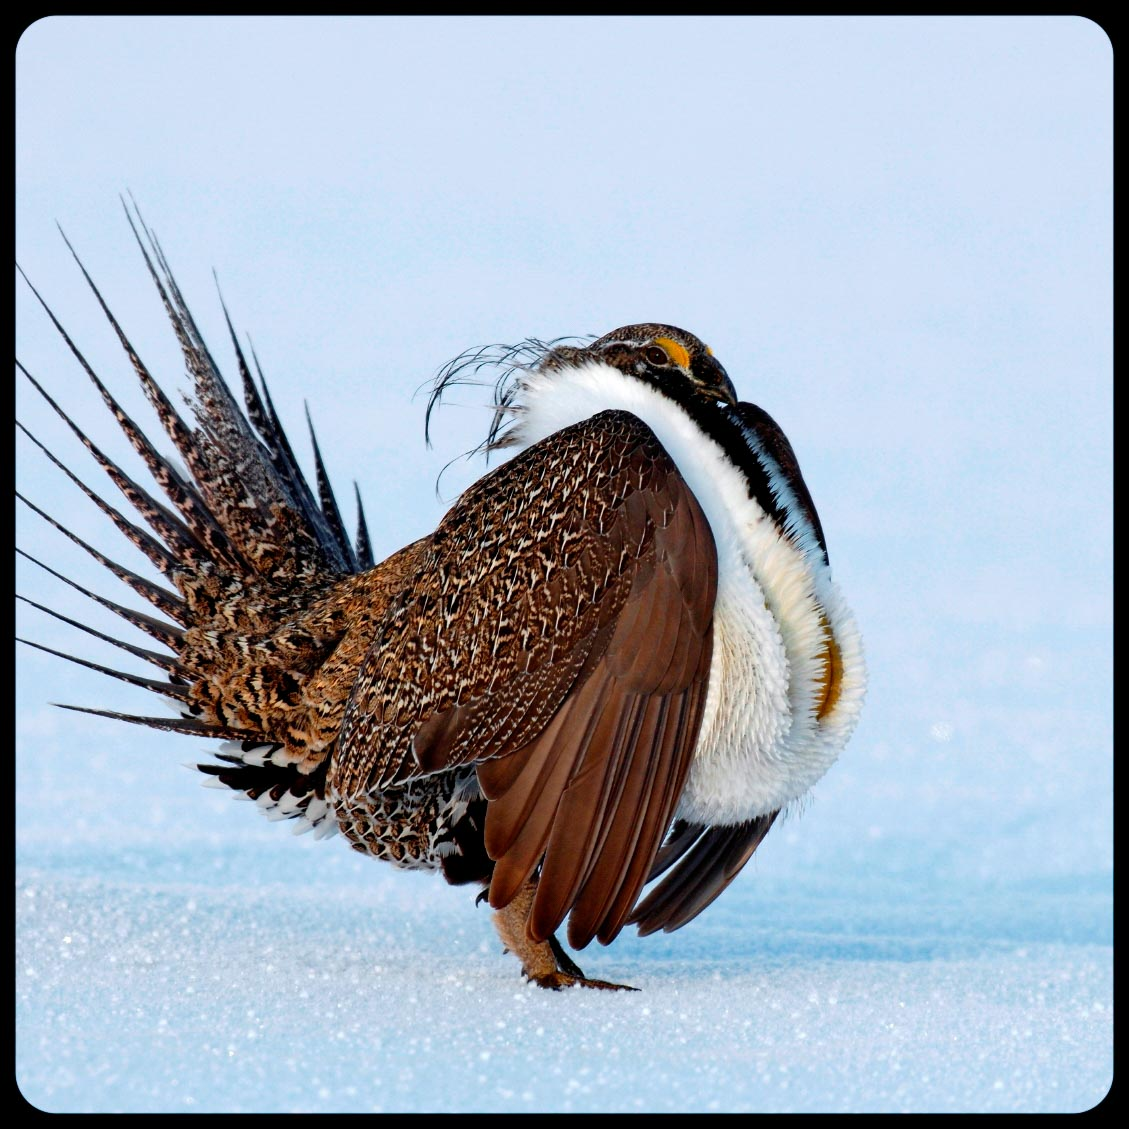
\includegraphics[width=0.7\linewidth]{images/sage-grouse} \end{center}

Greater Sage-Grouse (\emph{Centrocercus urophasianus}; hearafter sage-grouse) are ground nesting bird, distributed across the intermountain west with a range that across 11 states and 2 Canadian provinces. They are listed under the Canadian Species At Risk Act and of conservation concern throughout their distribution in the United States. There distribution is roughly consonant with the distribution of sagebrush (Artemisia sp.) habitat. The major negative impacts to sage-grouse are habitat loss, invasice species, and energy development across their range. Sage-grouse have a lek mating system in which males congregate at breeding sites (i.e., leks) each spring to compete for mating opportunities using elaborate `strutting' displays to attract females. There have been large efforts across their range to collect detailed ecological and population data - typically focused on lek sites. Approximately 35\% of the remaining sage-grouse occur in Wyoming. Long term monitoring data exists for many of the active leks across Wyoming are which are visited 1-3 times per lek season by biologists who count the number of males displaying at a lek. By convention, the highest number of males recorded across all visits is used as the lek size for a given year. These counts are considered a good index of overall population size and are used to assess trends in population numbers. This ongoing effort was started in 1948 and has resulted in a large dataset with thousands of leks where males have been counted and recorded each year. We will use some of these data to demonstrate approaches that can be used visualize and analyze a real ecological dataset. Given issues with data ownership and distribution, the data you will be working with are based on real data, but I have adjusted the data by introducing random variation into the counts and spatial lek locations. So the actual data you are working with have similar distributions and challenges associated with the real data, but but are not accurate in terms of lek locations and lek counts. Th

To get you started, we have provided a comma separated values file, which includes summary information on 718 leks from the southern half of the Wyoming. In the figure below you can see distribution of these leks in relation to their range (light grey) across this region.

\begin{center}\includegraphics[width=0.7\linewidth]{images/lek_locs_map} \end{center}

We have summarized the time-series of the leks described and mapped above, by calculating a variety of statistics on the time series form 1982-2013 (``140123wysg\_leks.csv''). Before beginning, get associated with this data by opening it in a text editor and excel. A description of data comprised for each column is listed below.

\begin{longtable}[]{@{}
  >{\raggedright\arraybackslash}p{(\columnwidth - 2\tabcolsep) * \real{0.4333}}
  >{\raggedright\arraybackslash}p{(\columnwidth - 2\tabcolsep) * \real{0.5667}}@{}}
\toprule\noalign{}
\begin{minipage}[b]{\linewidth}\raggedright
\textbf{Name}
\end{minipage} & \begin{minipage}[b]{\linewidth}\raggedright
\textbf{Description}
\end{minipage} \\
\midrule\noalign{}
\endhead
\bottomrule\noalign{}
\endlastfoot
lekid & name of lek \\
x & UTM easting coordinates \\
y & UTM northing coordibnates \\
area & name of the management ares (i.e., unit) \\
per\_miss & percent of years where lek counts were not conducted \\
per\_zero & percentage of years where no individual males were counted at a lek site \\
mean\_count & mean number of peak males counted across the time series \\
sd\_count & standard deviation of peak males counted across the time series \\
min\_count & minimum number of peak males counted across the time series \\
max\_count & maximum number of peak males counted across the time series \\
len\_road & length (m) of raods within 5 km radio of lek \\
mean\_ppt & mean of July, August, and September 1981-2010 total precipitation for climate zone surrounding lek \\
mean\_sage & mean sagebrush percent cover within 5 km radius of lek \\
mean\_herb & mean herbaceous percent cover within 5 km radius of lek \\
mean\_nest & mean nesting habitat suitability for sage-grouse (range: low(0) to high(1)) within 5km radius of lek \\
\end{longtable}

Once you are familiar with the data table, open Rstudio and setup a script file (do not forget to save the script file) that you will use to enter your commands throughout all exercises. You can translate your commands from the script to the concole (i.e., run your commands), by highlighting the commands and hitting control-enter on the keyboard. Make sure you input header information before you begin entering commands! It is also important to set your working directory to the directory where your data is saved before attempting to import the data.

\begin{Shaded}
\begin{Highlighting}[]
\CommentTok{\# set your working directory}
\NormalTok{leks }\OtherTok{\textless{}{-}} \FunctionTok{read.table}\NormalTok{(}\StringTok{"DATA/140123wysg\_leks.csv"}\NormalTok{, }\AttributeTok{sep=}\StringTok{","}\NormalTok{, }\AttributeTok{header=}\ConstantTok{TRUE}\NormalTok{,}\AttributeTok{quote=}\StringTok{""}\NormalTok{,}\AttributeTok{comment.char=}\StringTok{""}\NormalTok{, }
\AttributeTok{stringsAsFactors=}\ConstantTok{FALSE}\NormalTok{)  }\CommentTok{\# read in the data}
\FunctionTok{head}\NormalTok{(leks)  }\CommentTok{\# look at the first few observations}
\end{Highlighting}
\end{Shaded}

\begin{verbatim}
##              lekid        x       y area per_miss per_zero mean_count sd_count
## 1    D-Alkali Draw -1117044 2253178    D     46.9     50.0     34.529     17.6
## 2  D-Antelope Draw -1154827 2281868    D     28.1     40.6     52.391     45.4
## 3   D-Bench Corral -1148670 2278415    D     25.0     43.8     33.583     28.6
## 4       D-Big John -1099343 2250458    D     50.0     50.0     87.875     19.1
## 5 D-Big Sandy Flat -1088257 2252134    D     25.0     90.6      0.875      3.0
## 6  D-Billie's Draw -1152847 2275456    D     50.0     71.9     20.062     24.6
##   min_count max_count len_road mean_ppt mean_sage mean_herb mean_nest
## 1         0        67   172473     24.8      14.8      15.9     0.484
## 2         0       133   188797     28.2      16.5      16.7     0.525
## 3         0        87   219941     25.0      14.7      13.8     0.463
## 4        56       119   134197     24.9      14.5      14.3     0.434
## 5         0        14   185886     25.6      16.1      17.0     0.487
## 6         0        73   171083     26.5      16.0      13.4     0.555
\end{verbatim}

There are often issues when importing data. Typically these are caused by variables that contain character data. You can visually inspect your imported data using the \texttt{view()} function or by clicking the data table in your Environment in RStudio. It is useful to always use summary functions to ensure that everything imported as expected. Here we use two such functions.

\begin{Shaded}
\begin{Highlighting}[]
\FunctionTok{dim}\NormalTok{(leks)  }\CommentTok{\# provide dimensions of the data frame}
\end{Highlighting}
\end{Shaded}

\begin{verbatim}
## [1] 718  15
\end{verbatim}

\begin{Shaded}
\begin{Highlighting}[]
\FunctionTok{summary}\NormalTok{(leks)}
\end{Highlighting}
\end{Shaded}

\begin{verbatim}
##     lekid                 x                  y               area          
##  Length:718         Min.   :-1236354   Min.   :2043637   Length:718        
##  Class :character   1st Qu.:-1129942   1st Qu.:2122548   Class :character  
##  Mode  :character   Median : -980625   Median :2166752   Mode  :character  
##                     Mean   :-1012654   Mean   :2169603                     
##                     3rd Qu.: -910777   3rd Qu.:2208761                     
##                     Max.   : -790076   Max.   :2319509                     
##     per_miss       per_zero       mean_count       sd_count       min_count   
##  Min.   : 0.0   Min.   :  0.0   Min.   :  0.0   Min.   :  0.0   Min.   : 0.0  
##  1st Qu.: 0.0   1st Qu.: 46.9   1st Qu.:  2.6   1st Qu.:  5.8   1st Qu.: 0.0  
##  Median :12.5   Median : 65.6   Median : 10.3   Median : 11.7   Median : 0.0  
##  Mean   :19.9   Mean   : 62.2   Mean   : 16.6   Mean   : 15.6   Mean   : 1.2  
##  3rd Qu.:34.4   3rd Qu.: 81.2   3rd Qu.: 23.8   3rd Qu.: 20.8   3rd Qu.: 0.0  
##  Max.   :81.2   Max.   :100.0   Max.   :159.4   Max.   :104.5   Max.   :80.0  
##    max_count      len_road         mean_ppt      mean_sage       mean_herb   
##  Min.   :  0   Min.   : 35552   Min.   :15.8   Min.   : 0.00   Min.   : 3.8  
##  1st Qu.: 22   1st Qu.:122144   1st Qu.:20.9   1st Qu.: 8.00   1st Qu.: 8.2  
##  Median : 42   Median :155570   Median :23.9   Median : 9.99   Median :11.5  
##  Mean   : 56   Mean   :160325   Mean   :24.4   Mean   :10.19   Mean   :12.8  
##  3rd Qu.: 77   3rd Qu.:193281   3rd Qu.:27.4   3rd Qu.:12.27   3rd Qu.:16.3  
##  Max.   :350   Max.   :396330   Max.   :35.8   Max.   :19.76   Max.   :51.2  
##    mean_nest    
##  Min.   :0.000  
##  1st Qu.:0.101  
##  Median :0.162  
##  Mean   :0.198  
##  3rd Qu.:0.262  
##  Max.   :0.695
\end{verbatim}

It is useful to check the format of your data. We previously discussed some of the potential issues of storing columns as factors. Check to see if any columns are stored as factors. If needed re-import the data so that no columns are factors.

\hypertarget{summarizing-and-manipulating-data}{%
\subsection{Summarizing and manipulating data}\label{summarizing-and-manipulating-data}}

One of the key components to any analysis is the ability to summarize and manipulate your data. There are almost as many ways to accomplish common data summary tasks as there are users. We provided some of these basic functions earlier. However, in many cases you will want to summarize a data set using a grouping variable. For example, suppose we wish to determine the mean number of males counted within each of the management areas. One way this can be done using base R is with the \texttt{tapply()} function which applies a function to each group within a vector. To use \texttt{tapply} you supply i) a numeric vector of a data frame to be summarized (\texttt{X}; i.e., your variable of interest), ii) a grouping factor (\texttt{INDEX}), and iii) a function (\texttt{FUN}) to summarize the numeric vector:

\begin{Shaded}
\begin{Highlighting}[]
\FunctionTok{tapply}\NormalTok{(}\AttributeTok{X=}\NormalTok{leks}\SpecialCharTok{$}\NormalTok{mean\_count,}\AttributeTok{INDEX=}\NormalTok{leks}\SpecialCharTok{$}\NormalTok{area,}\AttributeTok{FUN=}\NormalTok{mean)}
\end{Highlighting}
\end{Shaded}

\begin{verbatim}
##     D     E     F     G     H 
## 30.96 28.49  8.53 16.68 13.14
\end{verbatim}

This example used \texttt{mean}; however, \texttt{tapply} can be used with any built in function (e.g., \texttt{sum()}, \texttt{sd()}, \texttt{length()}, \texttt{max()}, \texttt{min()}) or with a customized function of your own design. In addition to this flexibility, more than one grouping factor can be incorporated. For example, suppose we had some idea of a breakpoint between high and low quality nesting habitat for leks and we wanted to calculate a summary table describing the mean male counts for low and high suitability leks within each management area. To accomplish this we first need to create an additional variable, which groups the leks into `low' or `high' suitability groupings.

\begin{Shaded}
\begin{Highlighting}[]
\NormalTok{leks}\SpecialCharTok{$}\NormalTok{nest\_type}\OtherTok{\textless{}{-}}\StringTok{"low"}  \CommentTok{\# create a nesting suitablity variable }
\NormalTok{leks[leks}\SpecialCharTok{$}\NormalTok{mean\_nest}\SpecialCharTok{\textgreater{}}\FloatTok{0.3}\NormalTok{,}\StringTok{"nest\_type"}\NormalTok{]}\OtherTok{\textless{}{-}}\StringTok{"high"}  \CommentTok{\# change rows with values \textgreater{} 0.3 to \textquotesingle{}high\textquotesingle{}}
\NormalTok{leks\_sort}\OtherTok{\textless{}{-}}\NormalTok{leks[}\FunctionTok{order}\NormalTok{(leks}\SpecialCharTok{$}\NormalTok{nest\_type),] }\CommentTok{\#  sort data frame by nest\_type}
\end{Highlighting}
\end{Shaded}

Above we also use the \texttt{order()} function to sort the data frame by our new variable. Note that when we sort the data frame we create a new data frame, so the original data remains unmodified. View the sorted data frame to ensure the new variable is correctly assigned. After creating this variable you can use the \texttt{tapply} function with both the management area (area) and the newly created nest\_type variable:

\begin{Shaded}
\begin{Highlighting}[]
\NormalTok{lek\_summary}\OtherTok{\textless{}{-}}\FunctionTok{aggregate}\NormalTok{(}\AttributeTok{x=}\NormalTok{leks\_sort}\SpecialCharTok{$}\NormalTok{mean\_count,}\AttributeTok{by=}\FunctionTok{list}\NormalTok{(leks\_sort}\SpecialCharTok{$}\NormalTok{area,leks\_sort}\SpecialCharTok{$}\NormalTok{nest\_type), }\AttributeTok{FUN=}\NormalTok{mean)}
\NormalTok{lek\_summary}
\end{Highlighting}
\end{Shaded}

\begin{verbatim}
##    Group.1 Group.2     x
## 1        D    high 35.78
## 2        E    high 33.26
## 3        F    high 17.14
## 4        G    high 30.51
## 5        H    high  8.43
## 6        D     low 21.84
## 7        E     low 23.56
## 8        F     low  8.02
## 9        G     low 14.63
## 10       H     low 13.60
\end{verbatim}

The original data came in the form of a time series over multiple years. These summaries were created using the \texttt{apply()} function, which can be used to apply a function across rows (\texttt{MARGIN=1}) or down columns (\texttt{MARGIN=2}). To use these summaries, load the time series data using the \texttt{readtable} function.

\begin{Shaded}
\begin{Highlighting}[]
\NormalTok{lek\_ts}\OtherTok{\textless{}{-}}\FunctionTok{read.table}\NormalTok{(}\StringTok{"DATA/wysg\_peak\_males\_ts\_sub.csv"}\NormalTok{,}\AttributeTok{sep=}\StringTok{","}\NormalTok{,}\AttributeTok{header=}\ConstantTok{TRUE}\NormalTok{)}
\FunctionTok{head}\NormalTok{(lek\_ts)}
\end{Highlighting}
\end{Shaded}

\begin{verbatim}
##              lekid X2008 X2009 X2010 X2011 X2012 X2013
## 1   B-Blue Mesa 24    16    13    16    13     9     5
## 2  B-Grass Creek 2     0    17     4     5    12     7
## 3       B-Hoodoo 3    31    12    11     9     5     2
## 4   B-Logging Road    24    42    31    10    12    12
## 5          C-Innes    34    29    19    14    15    12
## 6 C-Upton-Fairview    11    13    12    10    17     9
\end{verbatim}

\begin{Shaded}
\begin{Highlighting}[]
\CommentTok{\# take mean across last 5 rows and add to new column}
\NormalTok{lek\_ts}\SpecialCharTok{$}\NormalTok{mean\_count}\OtherTok{\textless{}{-}}\FunctionTok{apply}\NormalTok{(}\AttributeTok{X=}\NormalTok{lek\_ts[,}\DecValTok{2}\SpecialCharTok{:}\DecValTok{7}\NormalTok{],}\AttributeTok{MARGIN=}\DecValTok{1}\NormalTok{,}\AttributeTok{FUN=}\NormalTok{mean) }
\FunctionTok{head}\NormalTok{(lek\_ts)}
\end{Highlighting}
\end{Shaded}

\begin{verbatim}
##              lekid X2008 X2009 X2010 X2011 X2012 X2013 mean_count
## 1   B-Blue Mesa 24    16    13    16    13     9     5       12.0
## 2  B-Grass Creek 2     0    17     4     5    12     7        7.5
## 3       B-Hoodoo 3    31    12    11     9     5     2       11.7
## 4   B-Logging Road    24    42    31    10    12    12       21.8
## 5          C-Innes    34    29    19    14    15    12       20.5
## 6 C-Upton-Fairview    11    13    12    10    17     9       12.0
\end{verbatim}

\hypertarget{data-visualization}{%
\chapter{Data Visualization}\label{data-visualization}}

\hypertarget{plotting-data}{%
\section{Plotting data}\label{plotting-data}}

In addition to statistical analysis and programming capabilities, R produces publishable quality graphics. Base R has the capacity to create excellent graphs; however, the syntax can sometimes feel a little clunky. Most recent graphing examples that you find online will make use of the wildly popular and exceptionally user-friendly package \texttt{ggplot2}. We will use this package throughout this book. There is a excellent book that describes all the details of this package called the \href{https://r-graphics.org/}{R Graphics Cookbook}. This chapter will introduce some basic level plotting and options and show you how to modify these options to customize plots. The next chapter will cover Data Exploration (i.e., summarizing and visualizing your data in order to inform your data analysis approach).

The first step is to install and load and the \texttt{ggplot2} package. We will also load a data set containing information on Eastern Fox Snakes (``efs\_growth.csv''). This data set investigates eastern fox snake (\emph{Pantherophis gloydi}) growth rates (``grate'') in two different regions in Ontario (``region''). Reptiles have indeterminate growth (i.e., grow throughout their entire lives), but their growth rates decline as they get older. The dataset also includes measurements on snout-to-vent length (``svl''; a proxy of age).

\begin{center}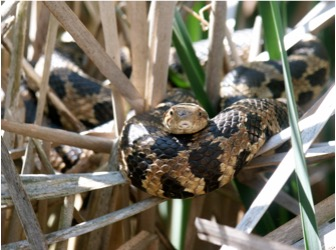
\includegraphics[width=0.7\linewidth]{images/EFS} \end{center}

\begin{Shaded}
\begin{Highlighting}[]
\FunctionTok{install.packages}\NormalTok{(}\StringTok{"ggplot2"}\NormalTok{)}
\end{Highlighting}
\end{Shaded}

\begin{Shaded}
\begin{Highlighting}[]
\FunctionTok{library}\NormalTok{(}\StringTok{"ggplot2"}\NormalTok{)}
\NormalTok{efs}\OtherTok{\textless{}{-}}\FunctionTok{read.csv}\NormalTok{(}\StringTok{"DATA/efs\_growth.csv"}\NormalTok{,}\AttributeTok{sep=}\StringTok{","}\NormalTok{,}\AttributeTok{header=}\ConstantTok{TRUE}\NormalTok{)}
\FunctionTok{head}\NormalTok{(efs)}
\end{Highlighting}
\end{Shaded}

\begin{verbatim}
##   Year days         ID region sex  SVL  grate
## 1 2007  333 4415685726  Essex   f 1270 -0.353
## 2 2010  369 4940181800  Essex   m  858  1.178
## 3 2009  730 4962583337  Essex   m 1042  0.340
## 4 2007  357 133637351a  Essex   f 1070  0.643
## 5 2007  415 133768254a  Essex   f  915  0.815
## 6 2008  711 134713166a  Essex   m  816  0.853
\end{verbatim}

\begin{Shaded}
\begin{Highlighting}[]
\FunctionTok{str}\NormalTok{(efs)}
\end{Highlighting}
\end{Shaded}

\begin{verbatim}
## 'data.frame':    207 obs. of  7 variables:
##  $ Year  : int  2007 2010 2009 2007 2007 2008 2008 2007 2009 2008 ...
##  $ days  : int  333 369 730 357 415 711 378 368 371 354 ...
##  $ ID    : chr  "4415685726" "4940181800" "4962583337" "133637351a" ...
##  $ region: chr  "Essex" "Essex" "Essex" "Essex" ...
##  $ sex   : chr  "f" "m" "m" "f" ...
##  $ SVL   : num  1270 858 1042 1070 915 ...
##  $ grate : num  -0.353 1.178 0.34 0.643 0.815 ...
\end{verbatim}

Imagine that we wanted to make a plot that displayed growth rate as a function of their snout-to-vent length (``svl''; a proxy of age). To plot with \texttt{ggplot}, we use the function \texttt{ggplot()}, which creates a coordinate system that we can then add layers to. The first argument for the \texttt{ggplot()} function is the data set that we want to use. In our case, the data set we want to use is `efs', which we loaded into our environment above. We then add one or more layers to our ggplot with a \texttt{geom\_} function. \texttt{Geoms} are geometric objects, like points, lines, or bars that we can add to our ggplot coordinate system. In this example, we will create a scatterplot with \texttt{geom\_point} comparing ``svl'' to ``grate''.

\begin{Shaded}
\begin{Highlighting}[]
\FunctionTok{ggplot}\NormalTok{(}\AttributeTok{data=}\NormalTok{efs,}\FunctionTok{aes}\NormalTok{(}\AttributeTok{x=}\NormalTok{SVL, }\AttributeTok{y=}\NormalTok{grate)) }\SpecialCharTok{+}
  \FunctionTok{geom\_point}\NormalTok{()}
\end{Highlighting}
\end{Shaded}

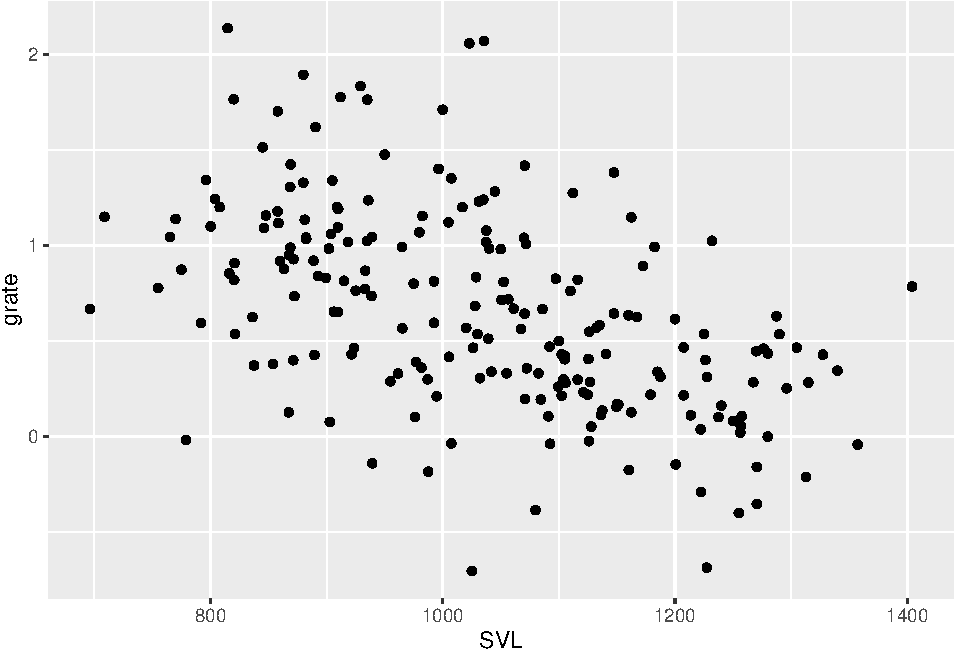
\includegraphics{series_files/figure-latex/unnamed-chunk-23-1.pdf}

As expected, we can see the negative relationship between snout-to-vent length (i.e, age) and growth. This helps us visualize the data, but we can improve the plot by adding better labels and making other manipulations to better visualize our data.

\hypertarget{manipulating-plots}{%
\section{Manipulating plots}\label{manipulating-plots}}

We can specify a number of parameters within the \texttt{geom\_} function. For example, we can modify the colour, transparency, shape, or size of the points. Don't forget that you can also use \texttt{?geom\_point} to understand what else you can do with this code or other \texttt{geom\_} functions.

\begin{Shaded}
\begin{Highlighting}[]
\FunctionTok{ggplot}\NormalTok{(}\AttributeTok{data=}\NormalTok{efs, }\FunctionTok{aes}\NormalTok{(}\AttributeTok{x=}\NormalTok{ SVL, }\AttributeTok{y=}\NormalTok{grate)) }\SpecialCharTok{+}   
    \FunctionTok{geom\_point}\NormalTok{(}\AttributeTok{colour =} \StringTok{"blue"}\NormalTok{,  }\CommentTok{\# change the colour of points}
               \AttributeTok{alpha =} \FloatTok{0.50}\NormalTok{,  }\CommentTok{\# change the transparency}
               \AttributeTok{shape =} \DecValTok{20}\NormalTok{,  }\CommentTok{\# change the shape of the point}
               \AttributeTok{size =} \DecValTok{2}\NormalTok{)  }\CommentTok{\# change the size of the point}
\end{Highlighting}
\end{Shaded}

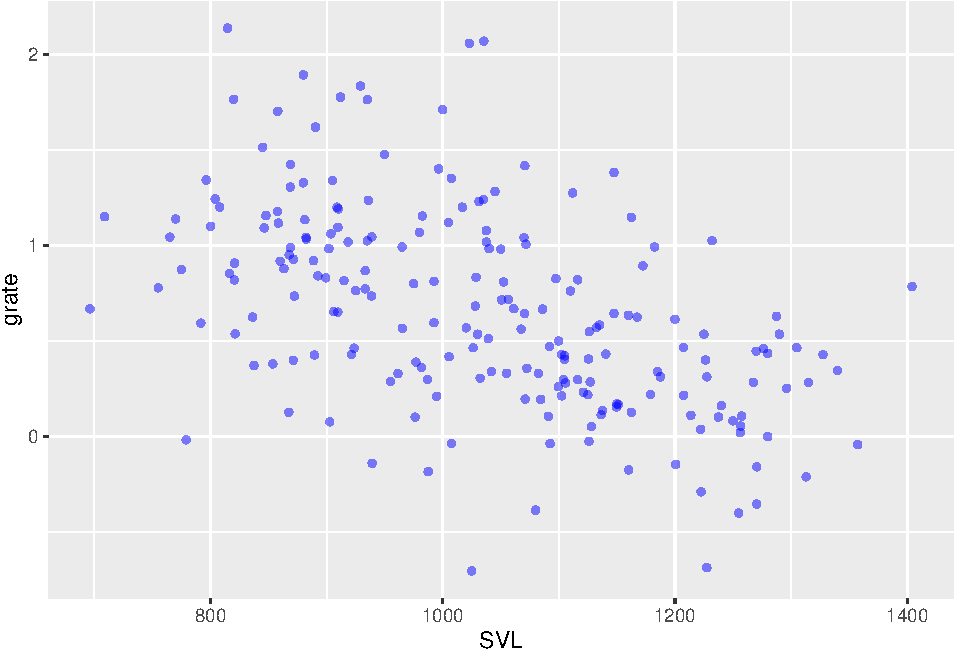
\includegraphics{series_files/figure-latex/unnamed-chunk-24-1.pdf}

R use numeric codes to represent different plot characters (\texttt{pch}), specified by the \texttt{shape} option in \texttt{ggplot2}. You can find indexes to these characters online or by typing \texttt{?pch} into the console. R defaults to the variable name. Frequently, these are difficult to decipher outside of your research group and need to be revised for publication and dissemination.

\begin{Shaded}
\begin{Highlighting}[]
\FunctionTok{ggplot}\NormalTok{(}\AttributeTok{data=}\NormalTok{efs, }\FunctionTok{aes}\NormalTok{(}\AttributeTok{x=}\NormalTok{ SVL, }\AttributeTok{y=}\NormalTok{grate)) }\SpecialCharTok{+}   
    \FunctionTok{geom\_point}\NormalTok{()}\SpecialCharTok{+}
    \FunctionTok{labs}\NormalTok{(}\AttributeTok{x =} \StringTok{"Snout{-}to{-}Vent Length (mm)"}\NormalTok{,}
         \AttributeTok{y =} \StringTok{"Growth Rate (mm/day)"}\NormalTok{) }\SpecialCharTok{+}
    \FunctionTok{scale\_x\_continuous}\NormalTok{(}\AttributeTok{breaks =} \FunctionTok{seq}\NormalTok{(}\DecValTok{0}\NormalTok{,}\DecValTok{1500}\NormalTok{,}\DecValTok{100}\NormalTok{))}\SpecialCharTok{+}
    \FunctionTok{scale\_y\_continuous}\NormalTok{(}\AttributeTok{breaks =} \FunctionTok{seq}\NormalTok{(}\SpecialCharTok{{-}}\DecValTok{1}\NormalTok{,}\DecValTok{3}\NormalTok{,}\FloatTok{0.5}\NormalTok{))}
\end{Highlighting}
\end{Shaded}

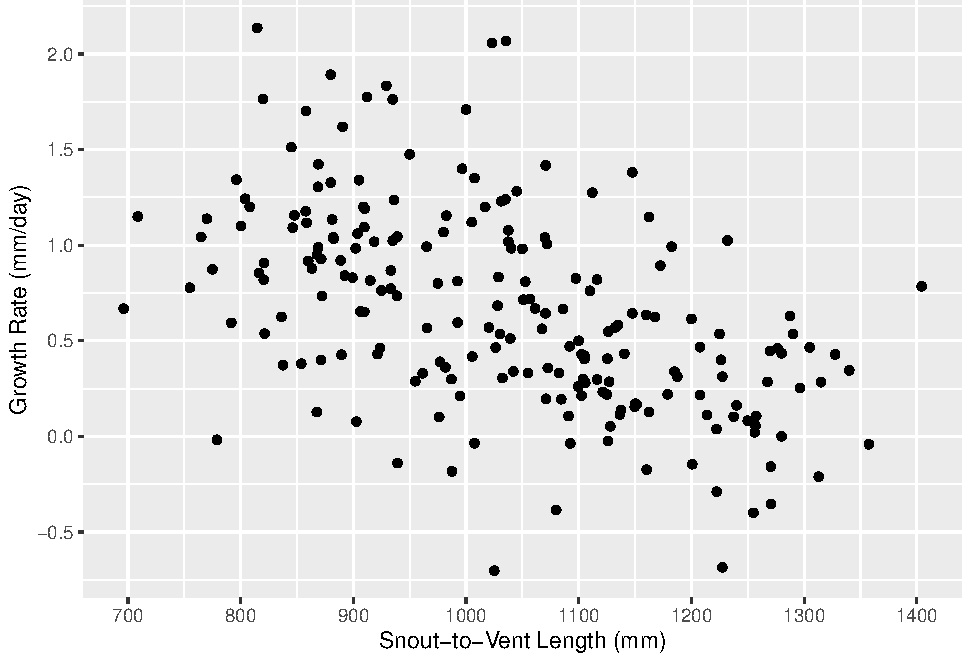
\includegraphics{series_files/figure-latex/unnamed-chunk-25-1.pdf}

All aspects of the graph are adjustable. It is often helpful to sketch your ideal plot first by hand and then figure out how plot it using \texttt{ggplot2}. You can also use \texttt{themes} in \texttt{ggplot2} to change the overall appearance of your plot and control all non-data display. There are many built-in themes and you can review their details \href{https://ggplot2.tidyverse.org/reference/ggtheme.html}{online}. You can also create your own \texttt{theme()} that you can replicate across analyses so that all your plots have a similar format. Themes are covered in Chapter 9 of the \href{https://r-graphics.org/}{R Graphics Cookbook}. A simple example of how to add a theme to your plot and a legend is here:

\begin{Shaded}
\begin{Highlighting}[]
\FunctionTok{ggplot}\NormalTok{(}\AttributeTok{data=}\NormalTok{efs, }\FunctionTok{aes}\NormalTok{(}\AttributeTok{x=}\NormalTok{ SVL, }\AttributeTok{y=}\NormalTok{grate, }\AttributeTok{colour=}\NormalTok{region)) }\SpecialCharTok{+}   
    \FunctionTok{geom\_point}\NormalTok{() }\SpecialCharTok{+}
    \FunctionTok{labs}\NormalTok{(}\AttributeTok{x =} \StringTok{"Snout{-}to{-}Vent Length (mm)"}\NormalTok{,  }\CommentTok{\# change x label}
         \AttributeTok{y =} \StringTok{"Growth Rate (mm/day)"}\NormalTok{,  }\CommentTok{\# change y label}
         \AttributeTok{colour =} \StringTok{"Region"}\NormalTok{) }\SpecialCharTok{+} \CommentTok{\# colour code points by Region}
    \FunctionTok{scale\_x\_continuous}\NormalTok{(}\AttributeTok{breaks =} \FunctionTok{seq}\NormalTok{(}\DecValTok{0}\NormalTok{,}\DecValTok{1500}\NormalTok{,}\DecValTok{100}\NormalTok{)) }\SpecialCharTok{+}  \CommentTok{\# specify x{-}scale}
    \FunctionTok{scale\_y\_continuous}\NormalTok{(}\AttributeTok{breaks =} \FunctionTok{seq}\NormalTok{(}\SpecialCharTok{{-}}\DecValTok{1}\NormalTok{,}\DecValTok{3}\NormalTok{,}\FloatTok{0.5}\NormalTok{)) }\SpecialCharTok{+}  \CommentTok{\# specify y{-}scale}
    \FunctionTok{theme\_classic}\NormalTok{()  }\CommentTok{\# specify theme}
\end{Highlighting}
\end{Shaded}

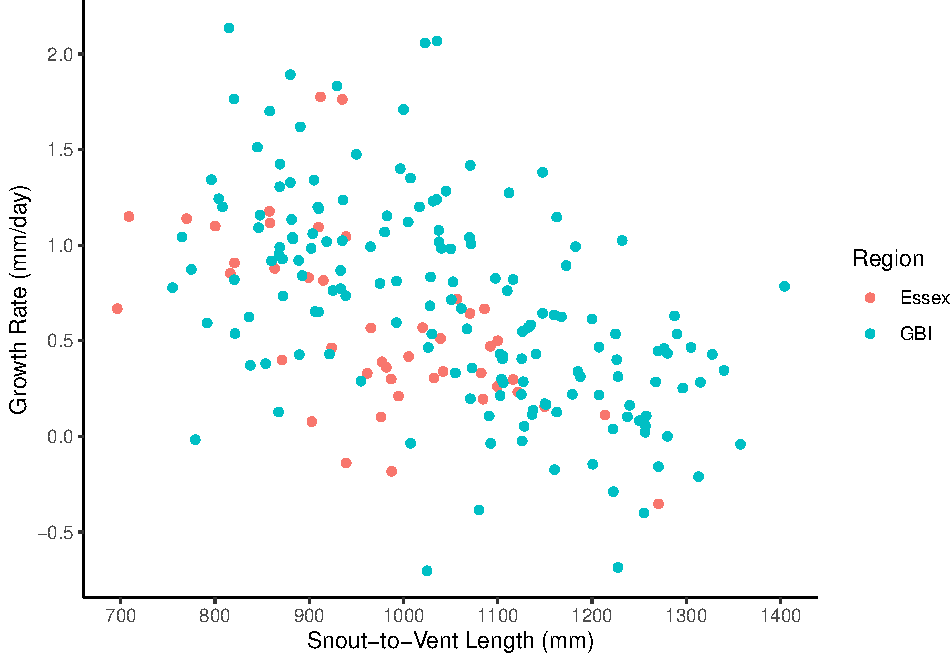
\includegraphics{series_files/figure-latex/unnamed-chunk-26-1.pdf}

\hypertarget{adding-low-level-plotting-functions}{%
\section{Adding low-level plotting functions}\label{adding-low-level-plotting-functions}}

Low-level plotting functions plot on already existing plots. For example suppose we had preformed a regression and wanted to add a regression line to our plot to further visualize the negative relationship between age and growth rate of Eastern fox snakes. We can do this using the geom\_smooth function to add the regression line to the plot.

\begin{Shaded}
\begin{Highlighting}[]
\FunctionTok{ggplot}\NormalTok{(}\AttributeTok{data=}\NormalTok{efs, }\FunctionTok{aes}\NormalTok{(}\AttributeTok{x=}\NormalTok{ SVL, }\AttributeTok{y=}\NormalTok{grate, }\AttributeTok{colour=}\NormalTok{region)) }\SpecialCharTok{+}      
        \FunctionTok{geom\_point}\NormalTok{()}\SpecialCharTok{+}   
        \FunctionTok{labs}\NormalTok{(}\AttributeTok{x =} \StringTok{"Snout{-}to{-}Vent Length (mm)"}\NormalTok{,        }
            \AttributeTok{y =} \StringTok{"Growth Rate (mm/day)"}\NormalTok{,}
            \AttributeTok{colour =} \StringTok{"Region"}\NormalTok{) }\SpecialCharTok{+}   
        \FunctionTok{scale\_x\_continuous}\NormalTok{(}\AttributeTok{breaks =} \FunctionTok{seq}\NormalTok{(}\DecValTok{0}\NormalTok{,}\DecValTok{1500}\NormalTok{,}\DecValTok{100}\NormalTok{))}\SpecialCharTok{+}
        \FunctionTok{scale\_y\_continuous}\NormalTok{(}\AttributeTok{breaks =} \FunctionTok{seq}\NormalTok{(}\SpecialCharTok{{-}}\DecValTok{1}\NormalTok{,}\DecValTok{3}\NormalTok{,}\FloatTok{0.5}\NormalTok{)) }\SpecialCharTok{+}   
        \FunctionTok{theme\_classic}\NormalTok{()}\SpecialCharTok{+}  \CommentTok{\# add a theme}
        \FunctionTok{geom\_smooth}\NormalTok{(}\AttributeTok{method=}\StringTok{"lm"}\NormalTok{)  }\CommentTok{\# add a regression line to our plot}
\end{Highlighting}
\end{Shaded}

\begin{verbatim}
## `geom_smooth()` using formula = 'y ~ x'
\end{verbatim}

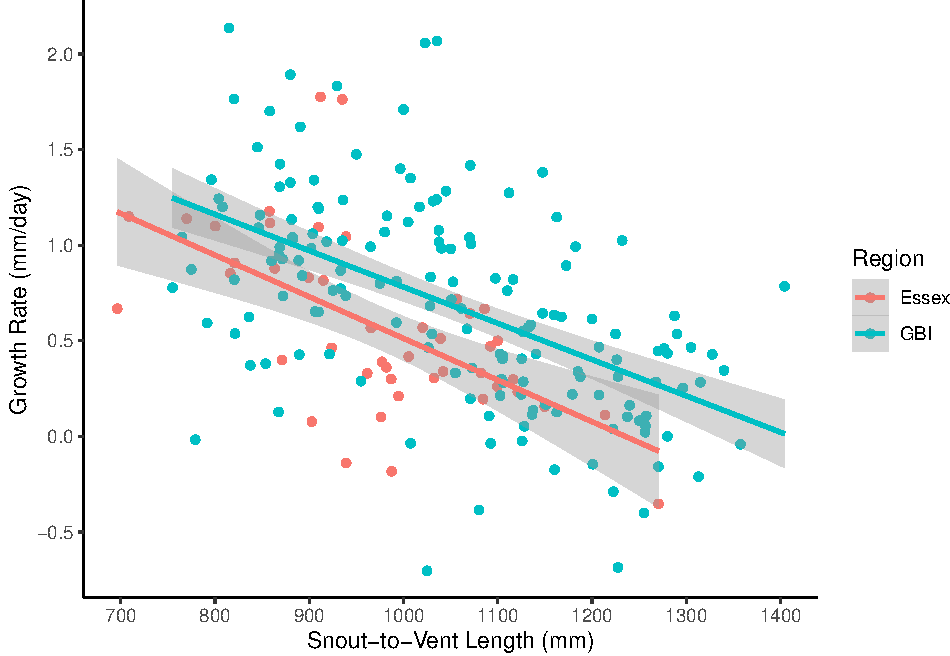
\includegraphics{series_files/figure-latex/unnamed-chunk-27-1.pdf}

\hypertarget{facet-plots}{%
\section{Facet plots}\label{facet-plots}}

When displaying data it is often useful to have multiple items highlighted on a single plot or to have a multi-panel plot for related data. Below we provide an example using this data to make a facet plot with the \texttt{facet\_grid} function. Again make sure you use help to understand what is happening with each line of code if it is not familiar to you (e.g, \texttt{?facet\_grid}).

Here, we are going to create a plot that compares growth rate with age for females and males at each different region. We will produce two separate plots for each region that compare males and females. We will also add regression lines.

\begin{Shaded}
\begin{Highlighting}[]
\FunctionTok{ggplot}\NormalTok{(}\AttributeTok{data=}\NormalTok{efs, }\FunctionTok{aes}\NormalTok{(}\AttributeTok{x=}\NormalTok{ SVL, }\AttributeTok{y=}\NormalTok{grate, }\AttributeTok{colour=}\NormalTok{sex)) }\SpecialCharTok{+}      
        \FunctionTok{geom\_point}\NormalTok{()}\SpecialCharTok{+}   
        \FunctionTok{labs}\NormalTok{(}\AttributeTok{x =} \StringTok{"Snout{-}to{-}Vent Length (mm)"}\NormalTok{,        }
            \AttributeTok{y =} \StringTok{"Growth Rate (mm/day)"}\NormalTok{,}
            \AttributeTok{colour =} \StringTok{"Region"}\NormalTok{) }\SpecialCharTok{+}   
        \FunctionTok{scale\_x\_continuous}\NormalTok{(}\AttributeTok{breaks =} \FunctionTok{seq}\NormalTok{(}\DecValTok{0}\NormalTok{,}\DecValTok{1500}\NormalTok{,}\DecValTok{100}\NormalTok{)) }\SpecialCharTok{+}
        \FunctionTok{scale\_y\_continuous}\NormalTok{(}\AttributeTok{breaks =} \FunctionTok{seq}\NormalTok{(}\SpecialCharTok{{-}}\DecValTok{1}\NormalTok{,}\DecValTok{3}\NormalTok{,}\FloatTok{0.5}\NormalTok{)) }\SpecialCharTok{+}   
        \FunctionTok{theme\_classic}\NormalTok{() }\SpecialCharTok{+}  \CommentTok{\# add a theme}
        \FunctionTok{geom\_smooth}\NormalTok{(}\AttributeTok{method=}\StringTok{"lm"}\NormalTok{) }\SpecialCharTok{+}  \CommentTok{\# add a regression line to our plot}
        \FunctionTok{facet\_grid}\NormalTok{(}\FunctionTok{vars}\NormalTok{(region))  }\CommentTok{\# add the facet grid for a variable of your choice}
\end{Highlighting}
\end{Shaded}

\begin{verbatim}
## `geom_smooth()` using formula = 'y ~ x'
\end{verbatim}

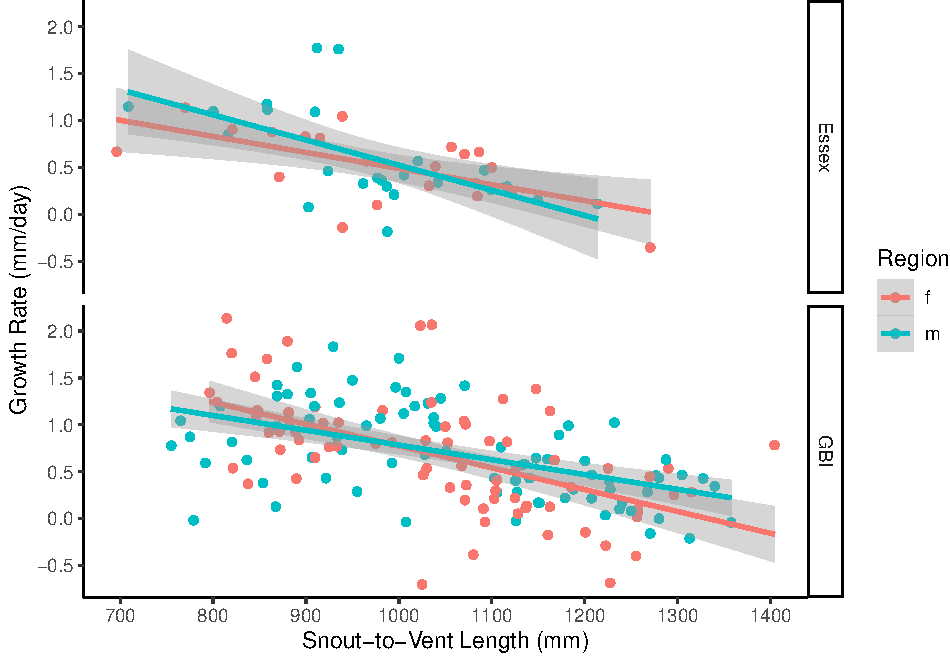
\includegraphics{series_files/figure-latex/unnamed-chunk-28-1.pdf}

Developing your plots in R is a great way to improve and maintain your R skills. This may seem like extra work compared to point-and-clicking your way through Excel to create a similar plot; but coding your plots allows for easy replication, update, sharing, and transparency. The code may look fairly complex to create a simple looking plot, but much of the code repeats and can be reused in future efforts.

The last thing we will do is save our plot to our working directory. You can do this through RStudio with the Export function in the plotting window; however, it is more useful to learn how to save with code so that you can make specifications to your figure size and file type. This can be accomplished using the \texttt{ggsave} function to output the figure with a specific size and file type. All journals have specifications regarding the size, file type, and resolution of figures for publication. The \texttt{ggsave} function an associated options ensures that you meet those criteria when submitting your research for publication.

\begin{Shaded}
\begin{Highlighting}[]
\FunctionTok{ggsave}\NormalTok{ (}\StringTok{"efs.figure.pdf"}\NormalTok{, }\AttributeTok{device =} \StringTok{"pdf"}\NormalTok{, }\AttributeTok{width =} \FloatTok{7.5}\NormalTok{, }\AttributeTok{height =} \DecValTok{5}\NormalTok{, }\AttributeTok{units =} \StringTok{"in"}\NormalTok{)}
\end{Highlighting}
\end{Shaded}

\hypertarget{data-exploration}{%
\chapter{Data Exploration}\label{data-exploration}}

Before conducting any statistical analysis you need to graphically explore your data. There are many packages within R to assist you with the process of data exploration. Many of the reasons behind data exploration and methodology are outlined in a review article in Methods in Ecology and Evolution by Zuur et al.~(2010) . We are pattern matching machines. We have evolved to visually detect patterns among the chaos. It is important to use that strength to visually inspect your data, understand its nuances, and allow that information to help inform your analyses in model structure.

We will cover general (and generlized) linear models in detail later in the course. However, it is necessary to introduce a simple model here to better explain why we recommend generating the plots in this chapter.

\[y_i = \beta_0 + \beta_1x_1 + \beta_2x_2 +  ...+ \beta_jx_i + \epsilon_i\]

In this model, we are trying to understand the relationship between a number of covariates (\(x_1, x_2\)) on the response variable of interest (\(y_i\)). The \(x_i\) and \(y_1\) represent actual data and measurements we have gathered. The model used that information to estimate the relationships among those variables. The shape and direction of the relationship between a particular \(x_i\) and our response variable \(y_i\) is describe by the slope estimates (e.g., \(\beta_1, \beta_2\)). In this relatively simple example, the model estimates two other parameters. The model intercept, \(\beta_0\) and the error term \(\epsilon_i\). This type of model can contain multiple \(x\) variables and both the \(y\) and \(x\) values may be discrete (i.e, values are individual, separated and distinct) or continuous (i.e., unbroken values between a range). The nature of the data (i.e., continuous or discrete) will change how you plot the variables. For this example, we will work with sage-grouse lek data.

One of the key questions driving much of wildlife ecology (honestly, much of most of ecology) is: how many animals are there? With the obvious follow up question of: why? Animal populations are influenced by a wide variety of environmental feature. Suppose we were interesting in determining if mean peak male counts (continuous \(y\) variable) were influenced by landscape or climate variables (continuous \(x\) variables) within the different management units (i.e., a discrete \(x\) variable) or within high and low nesting quality habitats (i.e., another discrete \(x\) variable). Before you begin with the code you need to load the lek data and add a grouping factor named ``nest\_type'' which divides the leks into high (\textgreater0.3) and low suitability (\textless=0.3). This was covered in previous chapters.

Unfortunately, in almost all field-base research, missing data is a reality. This is true of the sage-grouse data that we are using. Not all leks are surveyed every year.We will discuss how to deal with missing data in more depth in other parts of the course. For now, we want to remove leks from the analysis that have `too much' missing data. We have chosen a 50\% missing data as a cutoff for inclusion based on research by Dr.~Fedy exploring the impact of missing data and frequency of counts on lek population dynamic estimates. Therefore, we create a new lek dataset for exploration and analysis, by removing any leks where no individuals were counted across the whole time period (i.e., inactive leks) and those with more than 50 percent missing data. We are not going to do any statistical analysis on this dataset for now, but below we use graphical analysis to test a number of the statistical assumptions outlined in Zuur et al.~(2010).

\begin{Shaded}
\begin{Highlighting}[]
\FunctionTok{library}\NormalTok{(}\StringTok{\textquotesingle{}ggplot2\textquotesingle{}}\NormalTok{)}
\NormalTok{leks}\OtherTok{\textless{}{-}}\FunctionTok{read.csv}\NormalTok{(}\StringTok{"DATA/wysg\_peak\_males.csv"}\NormalTok{,}\AttributeTok{sep=}\StringTok{","}\NormalTok{,}\AttributeTok{header=}\ConstantTok{TRUE}\NormalTok{)}
\NormalTok{leks}\SpecialCharTok{$}\NormalTok{nest\_type}\OtherTok{\textless{}{-}}\StringTok{"low"}  \CommentTok{\# create a nesting suitablity variable}
\NormalTok{leks[leks}\SpecialCharTok{$}\NormalTok{mean\_nest}\SpecialCharTok{\textgreater{}}\FloatTok{0.3}\NormalTok{,}\StringTok{"nest\_type"}\NormalTok{]}\OtherTok{\textless{}{-}}\StringTok{"high"}  \CommentTok{\# change rows with values \textgreater{} 0.3 to \textquotesingle{}high\textquotesingle{}}
\NormalTok{leks\_sub}\OtherTok{\textless{}{-}}\NormalTok{leks[leks}\SpecialCharTok{$}\NormalTok{max\_count }\SpecialCharTok{!=} \DecValTok{0}\NormalTok{,]  }\CommentTok{\# subset with non{-}zero rows}
\NormalTok{leks\_sub}\OtherTok{\textless{}{-}}\NormalTok{leks\_sub[leks\_sub}\SpecialCharTok{$}\NormalTok{per\_miss }\SpecialCharTok{\textless{}} \DecValTok{50}\NormalTok{,]  }\CommentTok{\# subset for missing data}
\end{Highlighting}
\end{Shaded}

\hypertarget{outliers}{%
\section{Outliers}\label{outliers}}

Statistical outliers (i.e., data points that are distant from other data points in the dataset) can dominate the results of statistical analysis. Thus, outliers should be identified prior to statistical analysis so they can be removed or fixed if proper justification is found (e.g., error in data entry) or their effects on the analyses can be quantified if they are true biological outliers. As in Zuur et al., 2010 we use box plots and Cleveland dot plots on our y variable. You will see below that although there are no egregious outliers, some may warrant attention. To create the 2-panel plot, we will use the \texttt{cowplot} package. Don't forget to install and load the package before using the functions that require \texttt{cowplot}. Try and play around a bit with the \texttt{plot\_grid} function, see how you can create different plot displays.

\begin{Shaded}
\begin{Highlighting}[]
\CommentTok{\# To make the two panel plot, we first assign the two plots to objects in R}
\CommentTok{\# Create the boxplot}
\NormalTok{boxplot }\OtherTok{\textless{}{-}} \FunctionTok{ggplot}\NormalTok{(leks\_sub, }\FunctionTok{aes}\NormalTok{(}\AttributeTok{y=}\NormalTok{mean\_count))}\SpecialCharTok{+}   
            \FunctionTok{geom\_boxplot}\NormalTok{() }\SpecialCharTok{+}   
            \FunctionTok{labs}\NormalTok{(}\AttributeTok{y=}\StringTok{"Mean peak males"}\NormalTok{) }\SpecialCharTok{+}   
            \FunctionTok{theme\_bw}\NormalTok{()}

\CommentTok{\# Create the Cleveland dot chart}
\NormalTok{dotplot }\OtherTok{\textless{}{-}} \FunctionTok{ggplot}\NormalTok{(leks\_sub, }\FunctionTok{aes}\NormalTok{(}\AttributeTok{x=}\NormalTok{mean\_count, }\AttributeTok{y=}\FunctionTok{seq}\NormalTok{(}\DecValTok{1}\NormalTok{, }\FunctionTok{length}\NormalTok{(mean\_count),}\DecValTok{1}\NormalTok{))) }\SpecialCharTok{+}   
            \FunctionTok{geom\_point}\NormalTok{() }\SpecialCharTok{+}   
            \FunctionTok{labs}\NormalTok{(}\AttributeTok{x=}\StringTok{"Mean peak males"}\NormalTok{, }\AttributeTok{y =} \StringTok{"Order of the data"}\NormalTok{) }\SpecialCharTok{+}    
            \FunctionTok{theme\_bw}\NormalTok{()}

\CommentTok{\# Now plot them in the same window using the cowplot package}
\CommentTok{\#install.packages("cowplot", quiet=TRUE) \# code for installing package}
\FunctionTok{library}\NormalTok{(}\StringTok{"cowplot"}\NormalTok{, }\AttributeTok{quietly=}\ConstantTok{TRUE}\NormalTok{)}

\NormalTok{cowplot}\SpecialCharTok{::}\FunctionTok{plot\_grid}\NormalTok{(boxplot, dotplot)}
\end{Highlighting}
\end{Shaded}

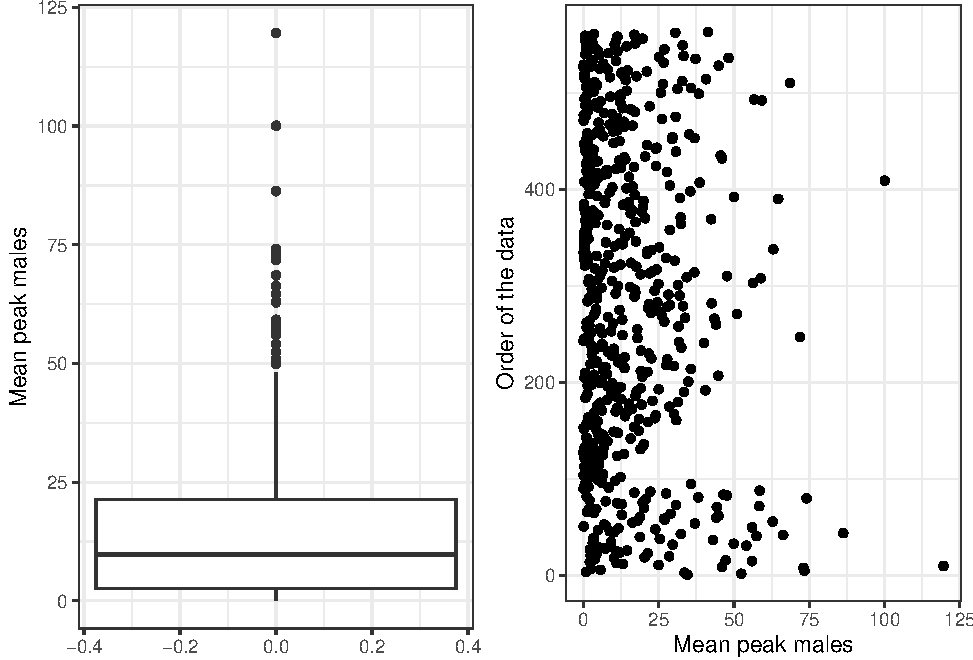
\includegraphics{series_files/figure-latex/unnamed-chunk-31-1.pdf}

In the previous chapter we created multipanel plots using the \texttt{facet\_grid} function. Here we used the cowplot to create a multipanel plot that displays the results from the two separate plots. Below we plot the mean peak male count and a number of landscape and climatic factors that are potentially having an effect on the number of males in a single plot. Before creating this plot, we create a subset matrix that can be used with the \texttt{facet\_wrap\ function}. Once we create the new susbet matrix of data that only contains the mean\_count and climate variables of interest, we will use code formatted based on the `tidyverse', which uses pipes (\texttt{\%\textgreater{}\%}), to format the dataset prior to plotting. The `tidyverse' is a popular data science group of packages and coding style used to `tidy' messy data to facilitate analysis and visualization. I use `tidyverse' occasionally, but I am not a diehard convert. If you want to delve deeper into the `tidyverse' I recommend the excellent book, \href{https://r4ds.hadley.nz/}{R for Data Science} which delves deep into the tidyverse universe and covers many important topics in data science. I take a pragmatic approach througout this book and the course. I do not really care what packages you use, as long as it works.

\begin{Shaded}
\begin{Highlighting}[]
\FunctionTok{library}\NormalTok{(}\StringTok{"tidyverse"}\NormalTok{, }\AttributeTok{quietly=}\ConstantTok{TRUE}\NormalTok{)}
\end{Highlighting}
\end{Shaded}

\begin{Shaded}
\begin{Highlighting}[]
\CommentTok{\# create a matrix by binding only the columns we are interested in}
\NormalTok{ex\_data}\OtherTok{\textless{}{-}}\FunctionTok{cbind}\NormalTok{(leks\_sub}\SpecialCharTok{$}\NormalTok{mean\_count,leks\_sub}\SpecialCharTok{$}\NormalTok{length\_road,leks\_sub}\SpecialCharTok{$}\NormalTok{mean\_sb,              }
\NormalTok{            leks\_sub}\SpecialCharTok{$}\NormalTok{mean\_herb,leks\_sub}\SpecialCharTok{$}\NormalTok{mean\_nest,leks\_sub}\SpecialCharTok{$}\NormalTok{mean\_ppt) }
\CommentTok{\# name the columns}
\FunctionTok{colnames}\NormalTok{(ex\_data)}\OtherTok{\textless{}{-}}\FunctionTok{c}\NormalTok{(}\StringTok{"mean\_count"}\NormalTok{,}\StringTok{"length\_road"}\NormalTok{,}\StringTok{"mean\_sb"}\NormalTok{,                      }
                    \StringTok{"mean\_herb"}\NormalTok{,}\StringTok{"mean\_nest"}\NormalTok{,}\StringTok{"mean\_ppt"}\NormalTok{)}
\CommentTok{\# create a new data set by converting the matrix to a data frame}
\NormalTok{ex\_data2 }\OtherTok{\textless{}{-}}\NormalTok{ ex\_data }\SpecialCharTok{\%\textgreater{}\%}   
    \FunctionTok{as.data.frame}\NormalTok{() }\SpecialCharTok{\%\textgreater{}\%}   
    \FunctionTok{gather}\NormalTok{(}\AttributeTok{key =} \StringTok{"variable"}\NormalTok{, }\AttributeTok{value =} \StringTok{"value"}\NormalTok{)    }
\CommentTok{\# plot the data}
\FunctionTok{ggplot}\NormalTok{(ex\_data2, }\FunctionTok{aes}\NormalTok{(}\AttributeTok{x=}\NormalTok{value, }\AttributeTok{y=}\FunctionTok{seq}\NormalTok{(}\DecValTok{1}\NormalTok{, }\FunctionTok{length}\NormalTok{(value),}\DecValTok{1}\NormalTok{))) }\SpecialCharTok{+}   
    \FunctionTok{geom\_point}\NormalTok{() }\SpecialCharTok{+}   
    \FunctionTok{labs}\NormalTok{(}\AttributeTok{x=}\StringTok{"Value of the variable"}\NormalTok{, }\AttributeTok{y =} \StringTok{"Order of the data"}\NormalTok{) }\SpecialCharTok{+}    
    \FunctionTok{theme\_bw}\NormalTok{() }\SpecialCharTok{+}   
    \FunctionTok{facet\_wrap}\NormalTok{(}\SpecialCharTok{\textasciitilde{}}\NormalTok{variable, }\AttributeTok{scales =} \StringTok{"free"}\NormalTok{)}
\end{Highlighting}
\end{Shaded}

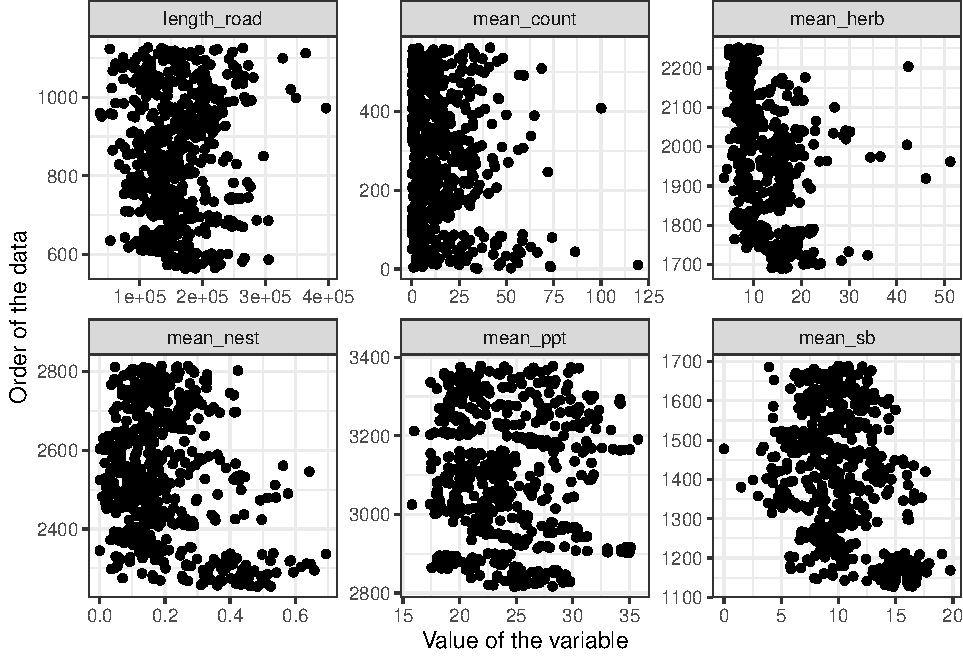
\includegraphics{series_files/figure-latex/unnamed-chunk-33-1.pdf}

\hypertarget{homoscedasticity-homegeneity-of-variance}{%
\section{Homoscedasticity (homegeneity of variance)}\label{homoscedasticity-homegeneity-of-variance}}

An important assumption in many statistical analysis is that variance (i.e., spread of data points) is similar between groups (e.g., sexes, different experimental treatments). Essentially, this assumption means that the residuals from a model have equal variance (homoscedasticity) for every fitted value and the predictors. Meeting this assumption ensures accurate calculation of standard errors for the parameter estiamtes. Thus, if we were interested in determining if the mean peak number of males for leks was different depending on the management area or the surrounding categorical nesting quality it would be important to explore this assumption. Here we see the true value of these graphing packages as they easily allow us to compare the distributions within one or more grouping factors using a box plot.

\begin{Shaded}
\begin{Highlighting}[]
\FunctionTok{ggplot}\NormalTok{(leks\_sub, }\FunctionTok{aes}\NormalTok{(}\AttributeTok{x=}\NormalTok{man\_area, }\AttributeTok{y=}\NormalTok{mean\_count))}\SpecialCharTok{+}
    \FunctionTok{geom\_boxplot}\NormalTok{()}\SpecialCharTok{+}
    \FunctionTok{labs}\NormalTok{(}\AttributeTok{x=}\StringTok{"Management Area"}\NormalTok{, }\AttributeTok{y=}\StringTok{"Mean peak males"}\NormalTok{)}\SpecialCharTok{+}
    \FunctionTok{theme\_bw}\NormalTok{()}\SpecialCharTok{+}
    \FunctionTok{facet\_wrap}\NormalTok{(}\SpecialCharTok{\textasciitilde{}}\NormalTok{nest\_type)}
\end{Highlighting}
\end{Shaded}

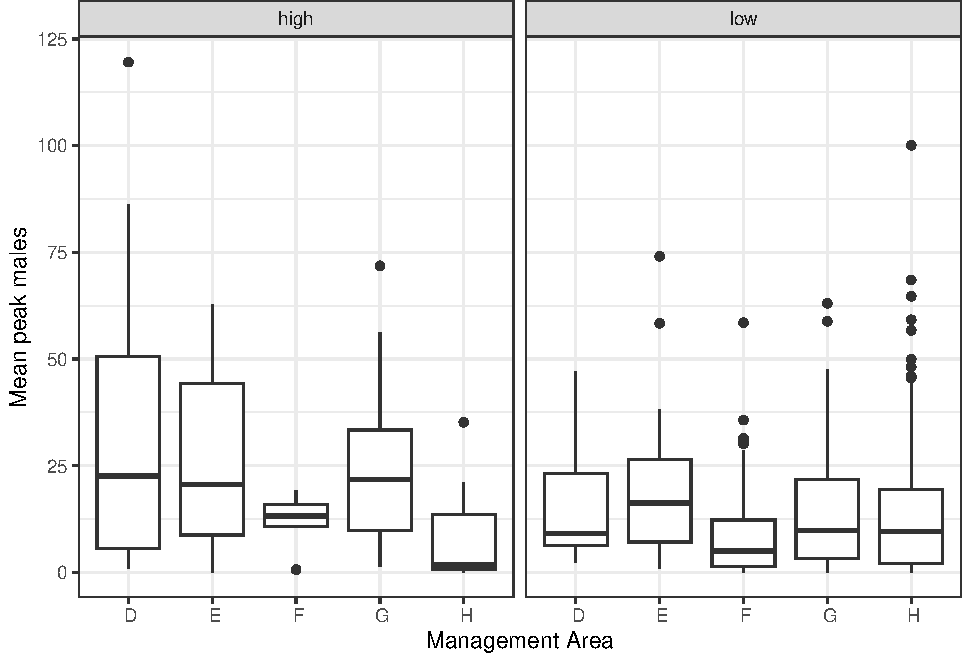
\includegraphics{series_files/figure-latex/unnamed-chunk-34-1.pdf}

Based on the plots above, it appears that we are violating the assumption of homogeneity of variance with some management areas having much lower variation in mean peak counts than others. We will discuss how to deal with this type of situation later in the course. But, these results suggest we may need to refine our research questions or account for these differences in our model development. Homoscedacity assumption determines how many variances are to be estimated: either one overall variance of the response variable, or several variances for different values of the explanatory variables. In the latter case, both the mean and the variance of the response variable change with the explanatory variables. We will get deeper into this when we discuss General(ized) Linear Models in later chapters particularly when we are discussing model fit.

\hypertarget{distribution-of-the-response-variable}{%
\section{Distribution of the response variable}\label{distribution-of-the-response-variable}}

An assumption in many statistical analyses is that your y variable is normally distributed. A simple way to assess this assumption is to visualize your data using a histogram. Here we use a two panel plot to plot both the mean peak number of males and the log(peak number of males), which is a common statistical transformation used to closer approximate a normal distribution.

\begin{Shaded}
\begin{Highlighting}[]
\NormalTok{hist\_mean }\OtherTok{\textless{}{-}} \FunctionTok{ggplot}\NormalTok{(leks\_sub, }\FunctionTok{aes}\NormalTok{(}\AttributeTok{x=}\NormalTok{mean\_count)) }\SpecialCharTok{+}                 
                \FunctionTok{geom\_histogram}\NormalTok{(}\AttributeTok{bins=}\DecValTok{30}\NormalTok{) }\SpecialCharTok{+}                 
                \FunctionTok{labs}\NormalTok{(}\AttributeTok{x=}\StringTok{"Mean number of males"}\NormalTok{, }\AttributeTok{y=}\StringTok{"Frequency"}\NormalTok{)}\SpecialCharTok{+}                 
                \FunctionTok{theme\_bw}\NormalTok{()}
\NormalTok{hist\_log }\OtherTok{\textless{}{-}} \FunctionTok{ggplot}\NormalTok{(leks\_sub, }\FunctionTok{aes}\NormalTok{(}\AttributeTok{x=}\FunctionTok{log}\NormalTok{(mean\_count))) }\SpecialCharTok{+}   
                \FunctionTok{geom\_histogram}\NormalTok{(}\AttributeTok{bins=}\DecValTok{30}\NormalTok{) }\SpecialCharTok{+}   
                \FunctionTok{labs}\NormalTok{(}\AttributeTok{x=}\StringTok{"Log(Mean number of males)"}\NormalTok{, }\AttributeTok{y=}\StringTok{"Frequency"}\NormalTok{)}\SpecialCharTok{+}   
                \FunctionTok{theme\_bw}\NormalTok{()                            }

\NormalTok{cowplot}\SpecialCharTok{::}\FunctionTok{plot\_grid}\NormalTok{(hist\_mean, hist\_log, }\AttributeTok{nrow=}\DecValTok{2}\NormalTok{)}
\end{Highlighting}
\end{Shaded}

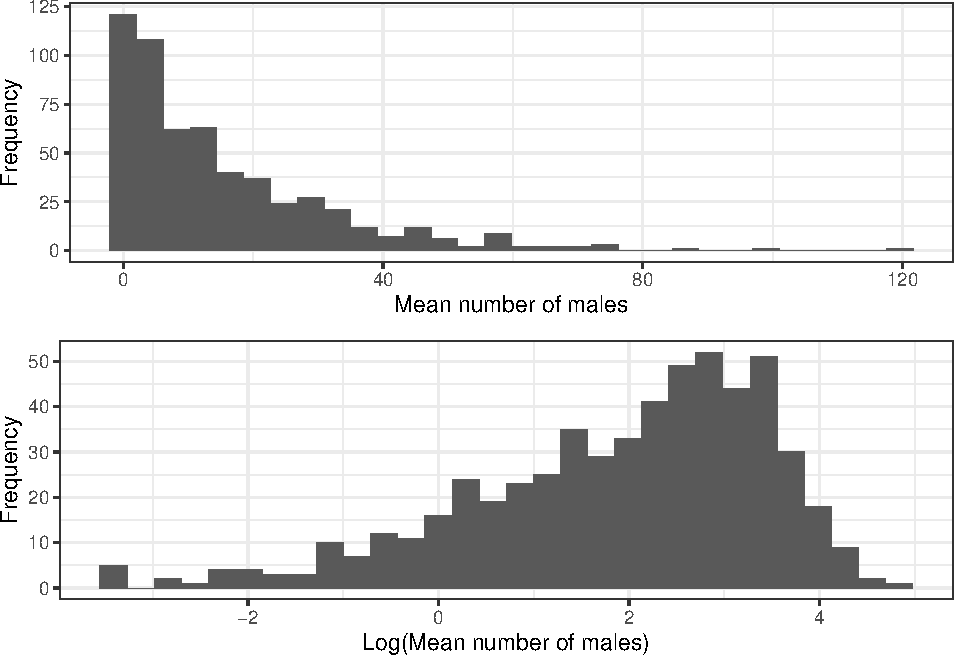
\includegraphics{series_files/figure-latex/unnamed-chunk-35-1.pdf}

Again the lattice package can also be useful for plotting multi-panel plots with multiple variables. Here we use the grouping factor (nest\_type) to look for normality within each nest group at the same time.

\begin{Shaded}
\begin{Highlighting}[]
\FunctionTok{ggplot}\NormalTok{(leks\_sub, }\FunctionTok{aes}\NormalTok{(}\AttributeTok{x=}\NormalTok{mean\_count))}\SpecialCharTok{+}
    \FunctionTok{geom\_histogram}\NormalTok{(}\AttributeTok{bins=}\DecValTok{30}\NormalTok{)}\SpecialCharTok{+}
    \FunctionTok{labs}\NormalTok{(}\AttributeTok{x=}\StringTok{"Mean number of males"}\NormalTok{, }\AttributeTok{y=}\StringTok{"Frequency"}\NormalTok{)}\SpecialCharTok{+}
    \FunctionTok{facet\_wrap}\NormalTok{(}\SpecialCharTok{\textasciitilde{}}\NormalTok{nest\_type)}\SpecialCharTok{+}
    \FunctionTok{theme\_bw}\NormalTok{()}
\end{Highlighting}
\end{Shaded}

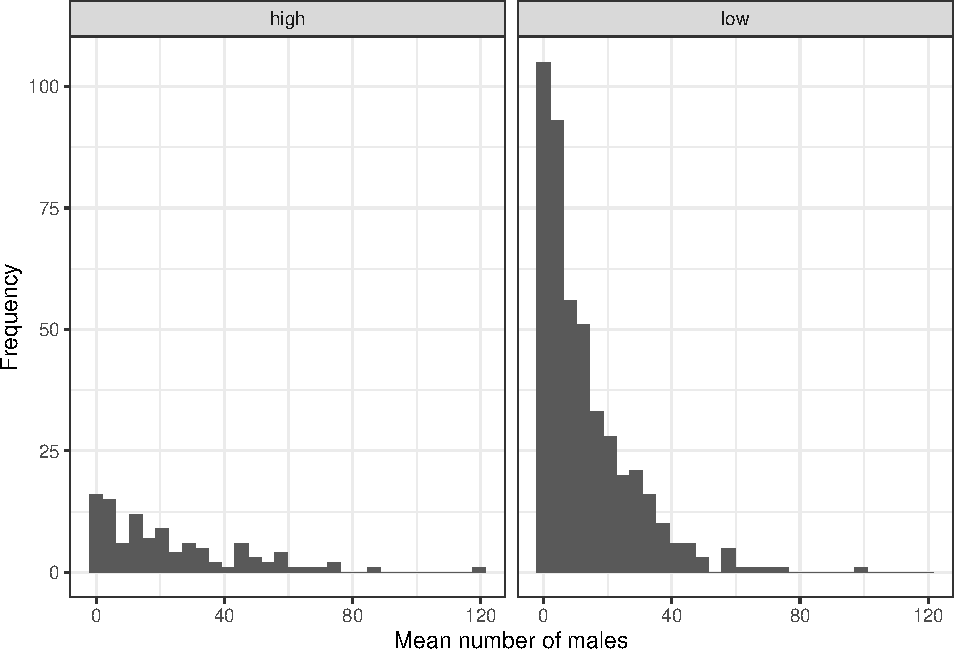
\includegraphics{series_files/figure-latex/unnamed-chunk-36-1.pdf}

\hypertarget{collinearity-among-x-variables}{%
\section{Collinearity among x variables}\label{collinearity-among-x-variables}}

When x variables (i.e., predictors) are highly correlated it is difficult to determine their independent effect on the y variable. Thus, it is always a good idea to determine the level of correlation among your predictors. Here we use a scatter plot to visualize the collinearity between the three landscape variables in the \texttt{ex\_data} dataframe. Here will use the \texttt{ggscatmat} function from the \texttt{GGally} package to visualize the correlation between variables. You will also notice in the plot that there is a strong positive correlation between sagebrush habitat and nesting quality, which is not surprising given the ecology of sage-grouse and their association with this habitat type.

\begin{Shaded}
\begin{Highlighting}[]
\CommentTok{\#install.packages("GGally", dependencies=TRUE, quiet=TRUE) }
\FunctionTok{library}\NormalTok{(}\StringTok{"GGally"}\NormalTok{, }\AttributeTok{quietly=}\ConstantTok{TRUE}\NormalTok{)}
\end{Highlighting}
\end{Shaded}

\begin{verbatim}
## Registered S3 method overwritten by 'GGally':
##   method from   
##   +.gg   ggplot2
\end{verbatim}

\begin{Shaded}
\begin{Highlighting}[]
\FunctionTok{ggscatmat}\NormalTok{(ex\_data, }\AttributeTok{columns =} \FunctionTok{c}\NormalTok{(}\DecValTok{3}\NormalTok{,}\DecValTok{4}\NormalTok{,}\DecValTok{5}\NormalTok{)) }\CommentTok{\#columns function selects specific comparisons}
\end{Highlighting}
\end{Shaded}

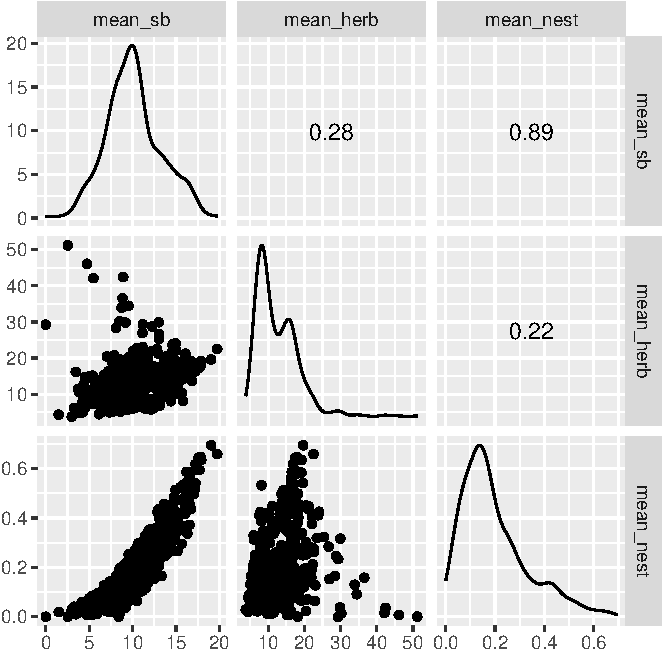
\includegraphics{series_files/figure-latex/unnamed-chunk-37-1.pdf}

\end{document}
